%%%%%%%%%%%%%%%%%%%%%%%%%%%%%%%%%%%%%%%%%%%%%%%%%%%%%%%%%%
%                                                                                      %
%         Bristol Project LaTex Template            %
%                                                                                      %
%%%%%%%%%%%%%%%%%%%%%%%%%%%%%%%%%%%%%%%%%%%%%%%%%%%%%%%%%%
%
%   Author: Alex Charles           Email: aep.charles@gmail.com
%
% -----------------------------------------------------------------------------------
%      PACKAGES & OTHER DOCUMENT CONFIGURATIONS
% -----------------------------------------------------------------------------------
\documentclass[11pt]{article}
\usepackage[utf8]{inputenc}
\usepackage[T1]{fontenc}
\usepackage[british]{babel}
% ----------NEW BIBLATEX BIBLIOGRAPHY-----------------------------------------------
\usepackage[backend=bibtex,style = ieee]{biblatex} % Upgrades Bibliography

\addbibresource{BibFile.bib} %%% For biblatex
%e.g to add page number \footfullcite[chapter, p.~215]{AAIB}
% This allows can use footfullcite commands
% Note urldate field must be in yyyy-mm-dd to work - use online type
% Remeber to use \printbibliography in the footer
% -----------------------------------------------------------------------------------
\usepackage{sectsty}
\usepackage{amssymb,amsmath}
\usepackage{ifxetex,ifluatex}  %<<<<<<<<< Edit FONT HERE
\ifnum 0\ifxetex 1\fi\ifluatex 1\fi=0 % if pdftex
  \usepackage[T1]{fontenc}
  \usepackage[utf8]{inputenc}
\else % if luatex or xelatex
  \ifxetex
    \usepackage{mathspec}
    \setmainfont{Avenir-Light}
  \else
  % Font Package for XeLatex
    \usepackage{fontspec}
    \setmainfont{Avenir-Light}
  \fi
  \defaultfontfeatures{Ligatures=TeX,Scale=MatchLowercase}
\fi
\usepackage[fit]{truncate} %Truncates headers that are too long
\usepackage{fancyhdr}
\usepackage{lastpage}
\usepackage{extramarks}
\usepackage{gensymb}
\usepackage{lipsum}
\usepackage{float}
\usepackage{graphicx}
\graphicspath{{TempImg/}{Img/}}%<<<<<<<<< Location of Template Images and Other Images, Add folders here
\usepackage{subfig}
\usepackage{wrapfig}
\usepackage[font ={small,it}]{caption}
\usepackage{amsfonts,amsthm} % Math packages
% \usepackage{cite}
% \usepackage[maxlevel=3]{csquotes}
%    \MakeAutoQuote{‘}{’}
%    \MakeAutoQuote*{“}{”} %corrects quote marks
\usepackage{enumitem} % resume numbered lists
\usepackage{multicol} %for mulitple colums in lists
\usepackage{geometry}
\usepackage{booktabs} %<<<<<<<<< Table drawing package
\usepackage[table,xcdraw]{xcolor} %<<<<<<<<< Table drawing package
\usepackage{svg}
\usepackage{scrextend} %call footnotes
\usepackage[colorlinks, linkcolor = black, citecolor = black, filecolor = black, urlcolor = blue]{hyperref} % Creates Hyperlinks for references - add [colorlinks] for coloured hyperlinks
\usepackage{changepage} %Allows Adjust width to be used for the document (indenting paragraphs)
\usepackage{pdfpages} %Allows Pdfpages to be added to the document use \includepdf[pages={1}]{myfile.pdf}
\usepackage{pdflscape} %Change Pages from Portrait to Landscape

%\usepackage[compact]{titlesec}
\usepackage{titlesec}
\titlespacing\section{0pt}{2pt plus 2pt minus 2pt}{0pt plus 2pt minus 2pt}
\titlespacing\subsection{0pt}{0pt plus 3pt minus 2pt}{-3pt plus 2pt minus 2pt}
\titlespacing\subsubsection{0pt}{0pt plus 2pt minus 2pt}{-4pt plus 2pt minus 2pt}
\titlespacing\subsubsubsection{0pt}{-6pt plus 2pt minus 2pt}{-4pt plus 2pt minus 2pt}
\setlength{\multicolsep}{-1pt plus 2.0pt minus 1.5pt}% 50% of original values

% \titlespacing*{\section}{0pt}{1.1\baselineskip}{\baselineskip}

\renewcommand*{\thefootnote}{\alph{footnote}} %%% Changes footnotes to letters
\usepackage[bottom]{footmisc} %%% Pushes footnote to bottom and to the margin

\DeclareCiteCommand{\footcite}[\mkbibfootnote]
{\usebibmacro{cite:init}%
\usebibmacro{prenote}}
{\usebibmacro{citeindex}%
\printtext[brackets]{\usebibmacro{cite:comp}}}
{\multicitedelim}
{\usebibmacro{cite:dump}%
\usebibmacro{postnote}}

\newenvironment{indentpara}{\begin{adjustwidth}{2cm}{}}{\end{adjustwidth}} %Declare adjust width wiht indentpara
\renewcommand{\labelitemii}{$\circ$}
\renewcommand{\labelitemiii}{$\diamond$}
\renewcommand{\labelitemiii}{$\cdot$}

% -----------------------------------------------------------------------------------
%                 Code
% -----------------------------------------------------------------------------------
\usepackage{listings}
\lstset{inputpath=Code/}
\usepackage{color}
\definecolor{mygreen}{RGB}{28,172,0} % color values Red, Green, Blue
\definecolor{mylilas}{RGB}{170,55,241}

\lstset{language=Matlab,%
    %basicstyle=\color{red},
    breaklines=true,%
    basicstyle=\small,
    morekeywords={matlab2tikz},
    keywordstyle=\color{blue},%
    morekeywords=[2]{1}, keywordstyle=[2]{\color{black}},
    identifierstyle=\color{black},%
    stringstyle=\color{mylilas},
    commentstyle=\color{mygreen},%
    showstringspaces=false,%without this there will be a symbol in the places where there is a space
    numbers=left,%
    numberstyle={\tiny \color{black}},% size of the numbers
    numbersep=9pt, % this defines how far the numbers are from the text
    emph=[1]{for,end,break},emphstyle=[1]\color{red}, %some words to emphasise
    %emph=[2]{word1,word2}, emphstyle=[2]{style},
}

%% To Add Code Use :
% \lstinputlisting{myfun.m}
%% To input a file or :
% \begin{figure}[h]
% \begin{lstlisting}[language=Matlab]
% \end{lstlisting}
% \catpion{code}
% \end{figure}


% -----------------------------------------------------------------------------------
%                 Quotes
% -----------------------------------------------------------------------------------

\usepackage{epigraph}
% \epigraphsize{\small}% Default
\setlength\epigraphwidth{12cm}
\setlength\epigraphrule{0pt}

\usepackage{etoolbox}
\apptocmd{\sloppy}{\hbadness 10000\relax}{}{}%%%% > Removes Url bibliography warnings
\makeatletter
\patchcmd{\epigraph}{\@epitext{#1}}{\itshape\@epitext{#1}}{}{}
\makeatother

%%%% > For Quotes Use \epigraph{"Quote"}{ - \textup{Author}, Book}

% -----------------------------------------------------------------------------------
%                   NAMES & CLASS DEFINITION %<<<<<<<<< INSERT DETAILS HERE
% -----------------------------------------------------------------------------------
\newcommand{\AssignmentTitle}{Part 2: Elevation Axis– Theory and Simulation with Control Requirements}
\newcommand{\ModuleTitle}{Sensors, Signals and Control}
\newcommand{\University}{University of Bristol}
\newcommand{\Faculty}{Faculty of Engineering}
\newcommand{\UniCrest}{crestbris.png}
\newcommand{\UniLogo}{logobris.png}%<<<<<<<<< Make Sure Files are in the Template
%\newcommand{\GroupName}{Group 2}
\newcommand{\StudentNameA}{Alex Charles}
\newcommand{\StudentNumberA}{ac13625}
\newcommand{\StudentNameB}{Akash Ramineni}
\newcommand{\StudentNumberB}{ar14120}
\newcommand{\SupervisorNameA}{Andres Marcos}
\newcommand{\SupervisorEmailA}{Andres.Marcos@bristol.ac.uk}
\newcommand{\SupervisorNameB}{Name}
\newcommand{\SupervisorEmailB}{email@gmail.com}

% -----------------------------------------------------------------------------------
%        PACKAGES FOR MARKDOWN CONVERSION - FOR USE If Using Markdown to Latex
% -----------------------------------------------------------------------------------
\usepackage{fixltx2e} % provides \textsubscript
% use upquote if available, for straight quotes in verbatim environments
\IfFileExists{upquote.sty}{\usepackage{upquote}}{}
% use microtype if available
\IfFileExists{microtype.sty}{%
\usepackage{microtype}
\UseMicrotypeSet[protrusion]{basicmath} % disable protrusion for tt fonts
}{}
\hypersetup{unicode=true,
            pdftitle={\AssignmentTitle},
            pdfauthor={\StudentNameA},
            pdfborder={0 0 0},
            breaklinks=true}
\urlstyle{same}  % don't use monospace font for urls
\usepackage{fancyvrb}
\VerbatimFootnotes % allows verbatim text in footnotes
\usepackage{longtable,booktabs}
\IfFileExists{parskip.sty}{%
\usepackage{parskip}
}{% else
\setlength{\parindent}{0pt}s
\setlength{\parskip}{6pt plus 2pt minus 1pt}
}
\setlength{\emergencystretch}{3em}  % prevent overfull lines
\providecommand{\tightlist}{%
  \setlength{\itemsep}{0pt}\setlength{\parskip}{0pt}}
% \setcounter{secnumdepth}{0}
% Redefines (sub)paragraphs to behave more like sections
\ifx\paragraph\undefined\else
\let\oldparagraph\paragraph
\renewcommand{\paragraph}[1]{\oldparagraph{#1}\mbox{}}
\fi
\ifx\subparagraph\undefined\else
\let\oldsubparagraph\subparagraph
\renewcommand{\subparagraph}[1]{\oldsubparagraph{#1}\mbox{}}
\fi

% -----------------------------------------------------------------------------------
%                   WORD COUTNER - for XeLaTex
% -----------------------------------------------------------------------------------
\usepackage{xesearch}
\newcounter{words}
\newenvironment{counted}{%
  \setcounter{words}{0}
  \SearchList!{wordcount}{\stepcounter{words}}
    {a?,b?,c?,d?,e?,f?,g?,h?,i?,j?,k?,l?,m?,
    n?,o?,p?,q?,r?,s?,t?,u?,v?,w?,x?,y?,z?}
  \UndoBoundary{'}
  \SearchOrder{p;}}{%
  \StopSearching}

% -----------------------------------------------------------------------------------
%                   MARGINS, HEADERS & FOOTERS
% -----------------------------------------------------------------------------------
 \geometry{
 left=20mm,
 right=20mm,
 top=20mm,
 bottom=20mm,
 }
\linespread{1.05}

\pagestyle{fancy}
\lhead{\includegraphics[width = 0.2\textwidth]{\UniLogo}}
% \chead{\AssignmentTitle}
% \rhead{}
\lfoot{\StudentNameA, \StudentNameB}
\cfoot{}
\rfoot{Page \thepage} %%%% note the footer is swapped when page numbering style changes
\renewcommand\headrulewidth{0.4pt}
\renewcommand\footrulewidth{0.4pt}

\setlength\parindent{0pt}

\newcommand{\horrule}[1]{\rule{\linewidth}{#1}}

% -----------------------------------------------------------------------------------
%               DOCUMENT STRUCTURE COMMANDS
% -----------------------------------------------------------------------------------
% To sort out the formatting of header and footer when a page...
% ... split occurs "within" a problem environment.
\newcommand{\enterProblemHeader}[1]{
\nobreak\extramarks{#1 (Cont.)}\nobreak
\nobreak\extramarks{#1}{}\nobreak
}
% To sort out the formatting of header and footer when a page...
% ... split occur "between" problem environments.
\newcommand{\exitProblemHeader}[1]{
\nobreak\extramarks{#1 (Cont.)}\nobreak
\nobreak\extramarks{#1}{}\nobreak
}

% -----------------------------------------------------------------------------------
\begin{document}

  \setlength{\abovedisplayskip}{-14pt}
  \setlength{\belowdisplayskip}{2pt}
  \setlength{\abovedisplayshortskip}{-14pt}
  \setlength{\belowdisplayshortskip}{2pt}

  \setlist[enumerate]{itemsep=-2mm}
  \setlist[itemize]{itemsep=-2mm}


%----------------------------------------------------------------------------------------
                                  %	TITLE PAGE FORMAT
%----------------------------------------------------------------------------------------
\pagenumbering{roman}
\begin{titlepage}

	\center % Center everything on the page
%----------------------------------------------------------------------------------------
%	HEADING SECTION
%----------------------------------------------------------------------------------------
		\usefont{OT1}{bch}{b}{n}
		\normalfont \normalsize \textsc{\University} \\ [10pt]
		\normalfont \normalsize \textsc{\Faculty} \\ [25pt]
%----------------------------------------------------------------------------------------
%	LOGO SECTION - Adds Univeristy Crest to the Report
%----------------------------------------------------------------------------------------
		\includegraphics[width = 0.2\textwidth]{\UniCrest}\\[0.5cm]
%----------------------------------------------------------------------------------------
%	HEADING SECTION
%----------------------------------------------------------------------------------------
		\normalfont \normalsize \textsc{\ModuleTitle} \\ [25pt]
%----------------------------------------------------------------------------------------
%	TITLE SECTION
%----------------------------------------------------------------------------------------
		\horrule{0.5pt} \\[0.4cm]
		\huge \textbf{\AssignmentTitle} \\
		\horrule{2pt} \\[0.5cm]
%----------------------------------------------------------------------------------------
%	HEADING SECTION
%----------------------------------------------------------------------------------------
%		\normalfont \normalsize \textsc{\GroupName} \\ [25pt]
%----------------------------------------------------------------------------------------
%	AUTHOR SECTION
%----------------------------------------------------------------------------------------
\begin{minipage}{0.4\textwidth}
\begin{flushleft} \large
\emph{Supervisors:}\\
% Change Name
\textbf{\SupervisorNameA}\\
% \textbf{\SupervisorNameB}
\end{flushleft}
\end{minipage}
~
\begin{minipage}{0.4\textwidth}
\begin{flushright} \large
\emph{Email:} \\
\SupervisorEmailA\\
% \SupervisorEmailB

\end{flushright}
\end{minipage}\\[1cm]

\begin{minipage}{0.4\textwidth}
\begin{flushleft} \large
\emph{Authors:}\\
	\textbf{\StudentNameA}\\
  \textbf{\StudentNameB}
\end{flushleft}
\end{minipage}
~
\begin{minipage}{0.4\textwidth}
\begin{flushright} \large
\emph{Candidate Number:} \\
(\StudentNumberA)\\
(\StudentNumberB)
\end{flushright}
\end{minipage}\\[2cm]

%----------------------------------------------------------------------------------------
%	DATE SECTION
%----------------------------------------------------------------------------------------
\textit{{\large \today}}\\[1cm] % Date, change the \today to a set date if you want to be precise
%----------------------------------------------------------------------------------------
\vfill % Fill the rest of the page with whitespace
\end{titlepage}

% \setcounter{page}{3}

\newpage


% -----------------------------------------------------------------------------------
%                             	 ABSTRACT
% -----------------------------------------------------------------------------------

% \addcontentsline{toc}{section}{Abstract}
% \begin{abstract}
%
% \end{abstract}
% -----------------------------------------------------------------------------------
%                              TABLE OF CONTENTS
% -----------------------------------------------------------------------------------

% \tableofcontents


% \newpage

% \addcontentsline{toc}{section}{List of Tables}
% \listoftables
% \addcontentsline{toc}{section}{List of Figures}
% \listoffigures
% \addcontentsline{toc}{section}{List of Acronyms}
% \section*{List of Acronyms}\label{acronyms}
% \textbf{BRB}: Be Right Back \\


% \newpage

% \addcontentsline{toc}{section}{Acknowledgements}
% \section*{Acknowledgements}\label{acknowledgements}

% \addcontentsline{toc}{section}{Declaration}
% \section*{Declaration}\label{declartion}
% I hereby declare that this report entitled “\AssignmentTitle” submitted to Bristol University, is a record of an original work completed by myself.\\

% \newpage

%% -----------------------------------------------------------------------------------
%%                          	  INTRODUCTION
%% -----------------------------------------------------------------------------------
\clearpage
\rfoot{Page \thepage\ of \pageref{LastPage}}
\pagenumbering{arabic}
\begin{counted} %<<<<<<<<<<<<<<STARTS WORD COUNTER
\section{P-I-D analysis}\label{p-i-d-analysis}

This report introduces the effects of proportional, derivative and
integral gains, implemented by a conventional PID controller on a
Quanser's behaviour
\footnote{See Control Coursework Part 1 for a derivation of the open-loop second order transfer functions for the Quanser elevation axis}.
This is assessed using time-domain and root locus results. A closed loop
PID controller, is used to reduce tracking error (\(e\)) between the
control input and the observed output \cite{ControlT54:online}. Through
correctly tuning the PID controller, it is desirable to achieve a sharp
response to a unit step input. The simulated results were verified by
theory predictions.

\subsection{Proportional Feedback
Controller}\label{proportional-feedback-controller}

\begin{wrapfigure}{r}{0.5\textwidth}
\centering
\vspace{-35pt} % Space added to the top of the image
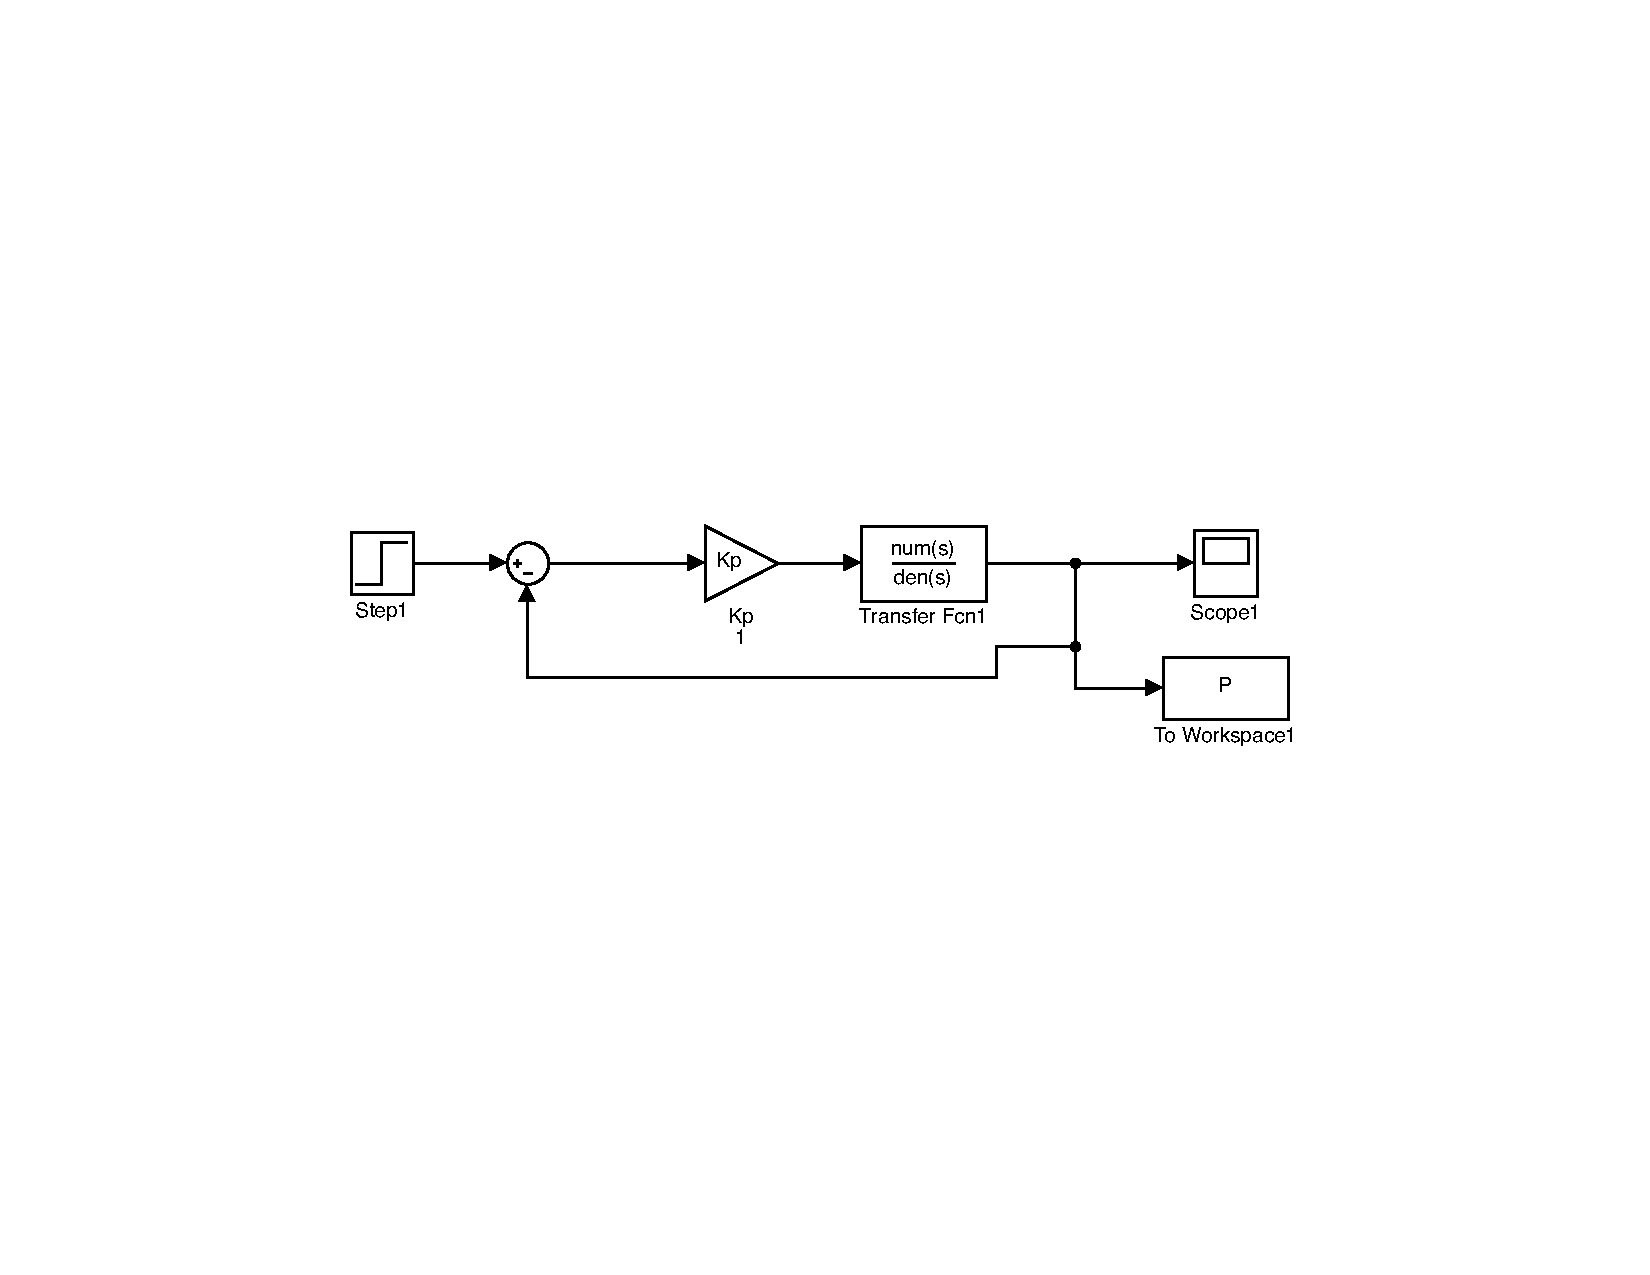
\includegraphics[trim = 0 0 0 0, clip, width=0.5\textwidth]{Psim.pdf}
\vspace{-25pt}
\caption{Proportional Feedback Controller}
\label{Psim}
\vspace{-15pt}
\end{wrapfigure}

Proportional gain control uses the \emph{Present} state of a plant to
error correct. The correction applied is proportional to the deviation
from the desired state of the plant. The result causes a highly
oscillatory system response, as the present error evaluates the
instantaneous state of the plant only. The simulation shown in Figure
\ref{Psim} found the effect of varying proportional gain (\(K_p\)) for
the Quanser transfer function. The simulation executed an iterative loop
with varying \(K_p\) from 0 to 0.1 in increments of 0.01. Figure
\ref{pres} shows the time domain response of increasing \(K_p\). When
\(K_p = 0\), a flat line was observed as there is no signal passing
through the plant. By extending proportional gain, the correction factor
became larger, increasing amplitude for higher \(K_p\) gains. The
\texttt{stepinfo()} function revealed that an increase in \(K_p\),
reduced both rise time and steady-state error while raising overshoot.

The root locus plot in \ref{pzp} allows observation of s-domain features
with varying proportional gain. For pure variation in proportional gain,
the (stable) poles are restricted to the same distance from the
imaginary axis. By increasing \(K_p\) the poles moved away from the real
axis in both directions, increasing natural-frequency (\(\omega_n\)) and
decreasing damping ratio \(\zeta\). The result verifies the observation
noted in the time domain response, as increased natural frequency will
lead to greater oscillatory behaviour, and reduced damping ratio
increases the overshoot.

\begin{figure}[H]
\centering
\begin{minipage}{.455\textwidth}
 \centering
 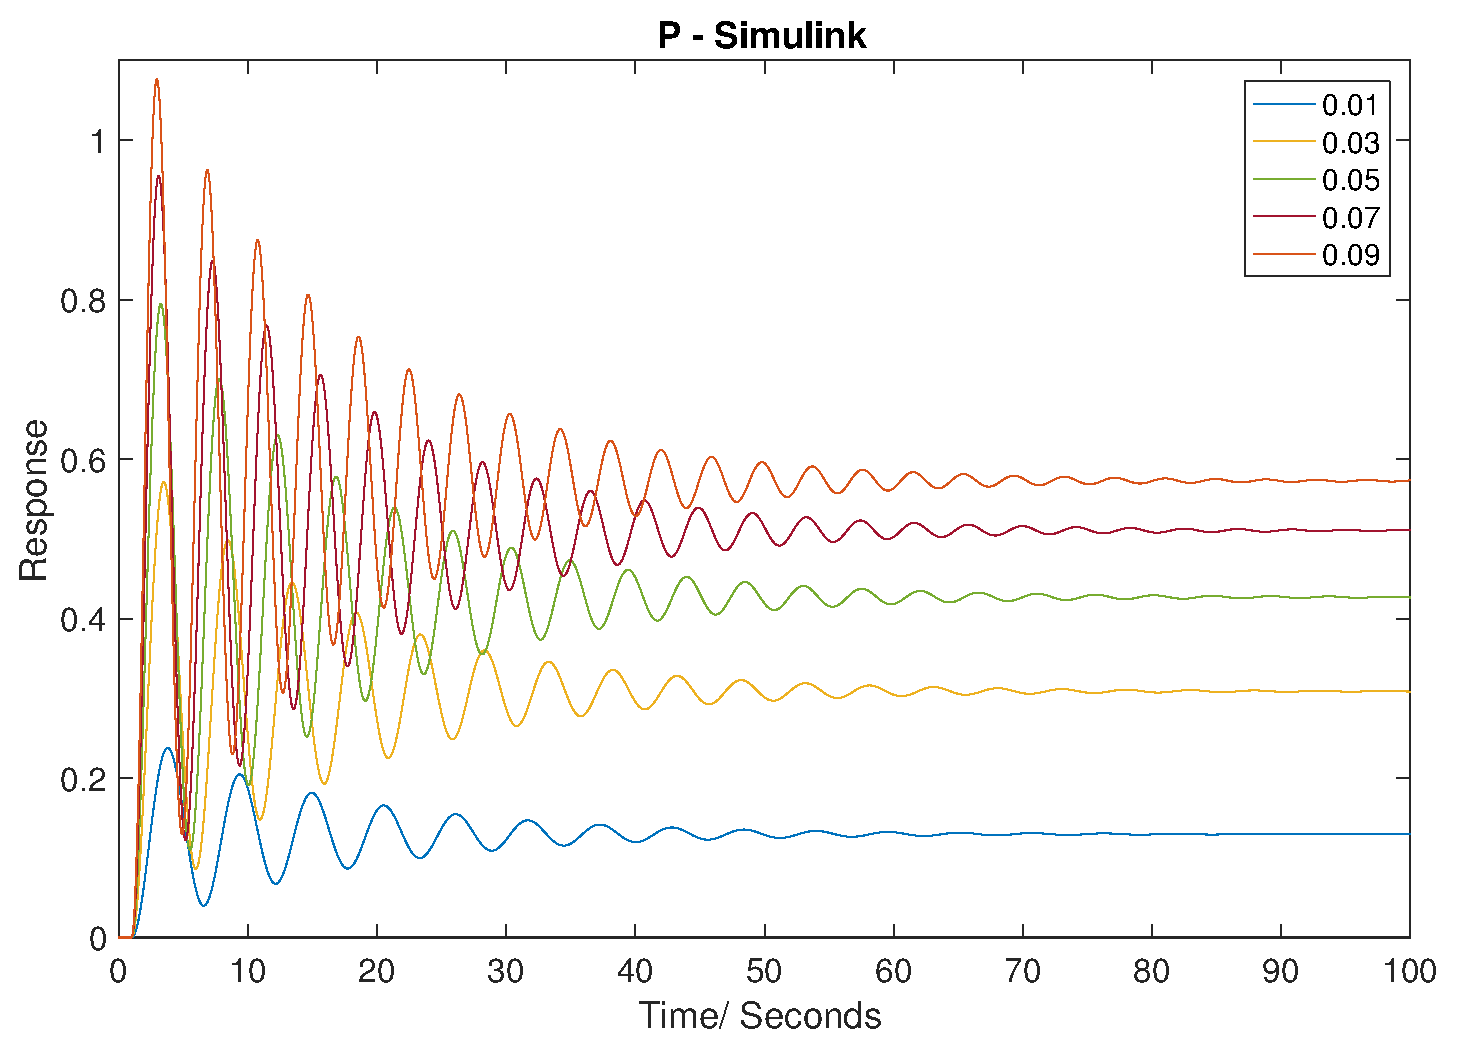
\includegraphics[trim = 0 0 0 0, clip, width=1\textwidth]{pres.eps}
 \caption{Response of Varying $K_p$}
 \label{pres}
\end{minipage}
\hfill
\begin{minipage}{.5\textwidth}
\centering
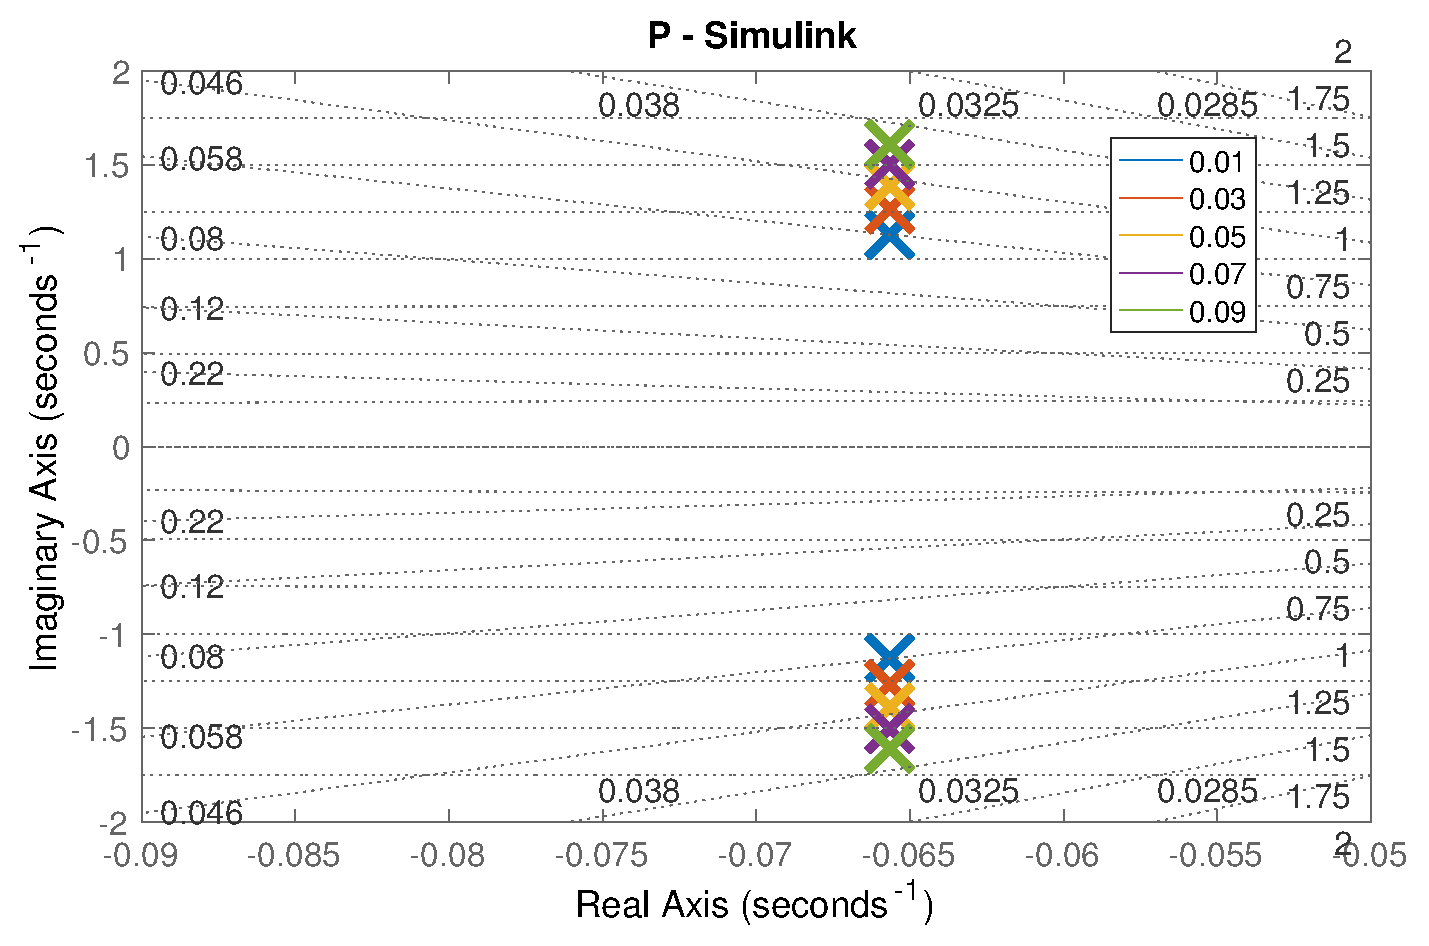
\includegraphics[trim = 0 0 0 0, clip, width=1\textwidth]{pzp.eps}
\caption{Poles of Varying $K_p$}
\label{pzp}
\end{minipage}
\vspace{-20pt}
\end{figure}

\subsection{Derivative Feedback
Controller}\label{derivative-feedback-controller}

\begin{wrapfigure}{r}{0.6\textwidth}
\centering
\vspace{-35pt} % Space added to the top of the image
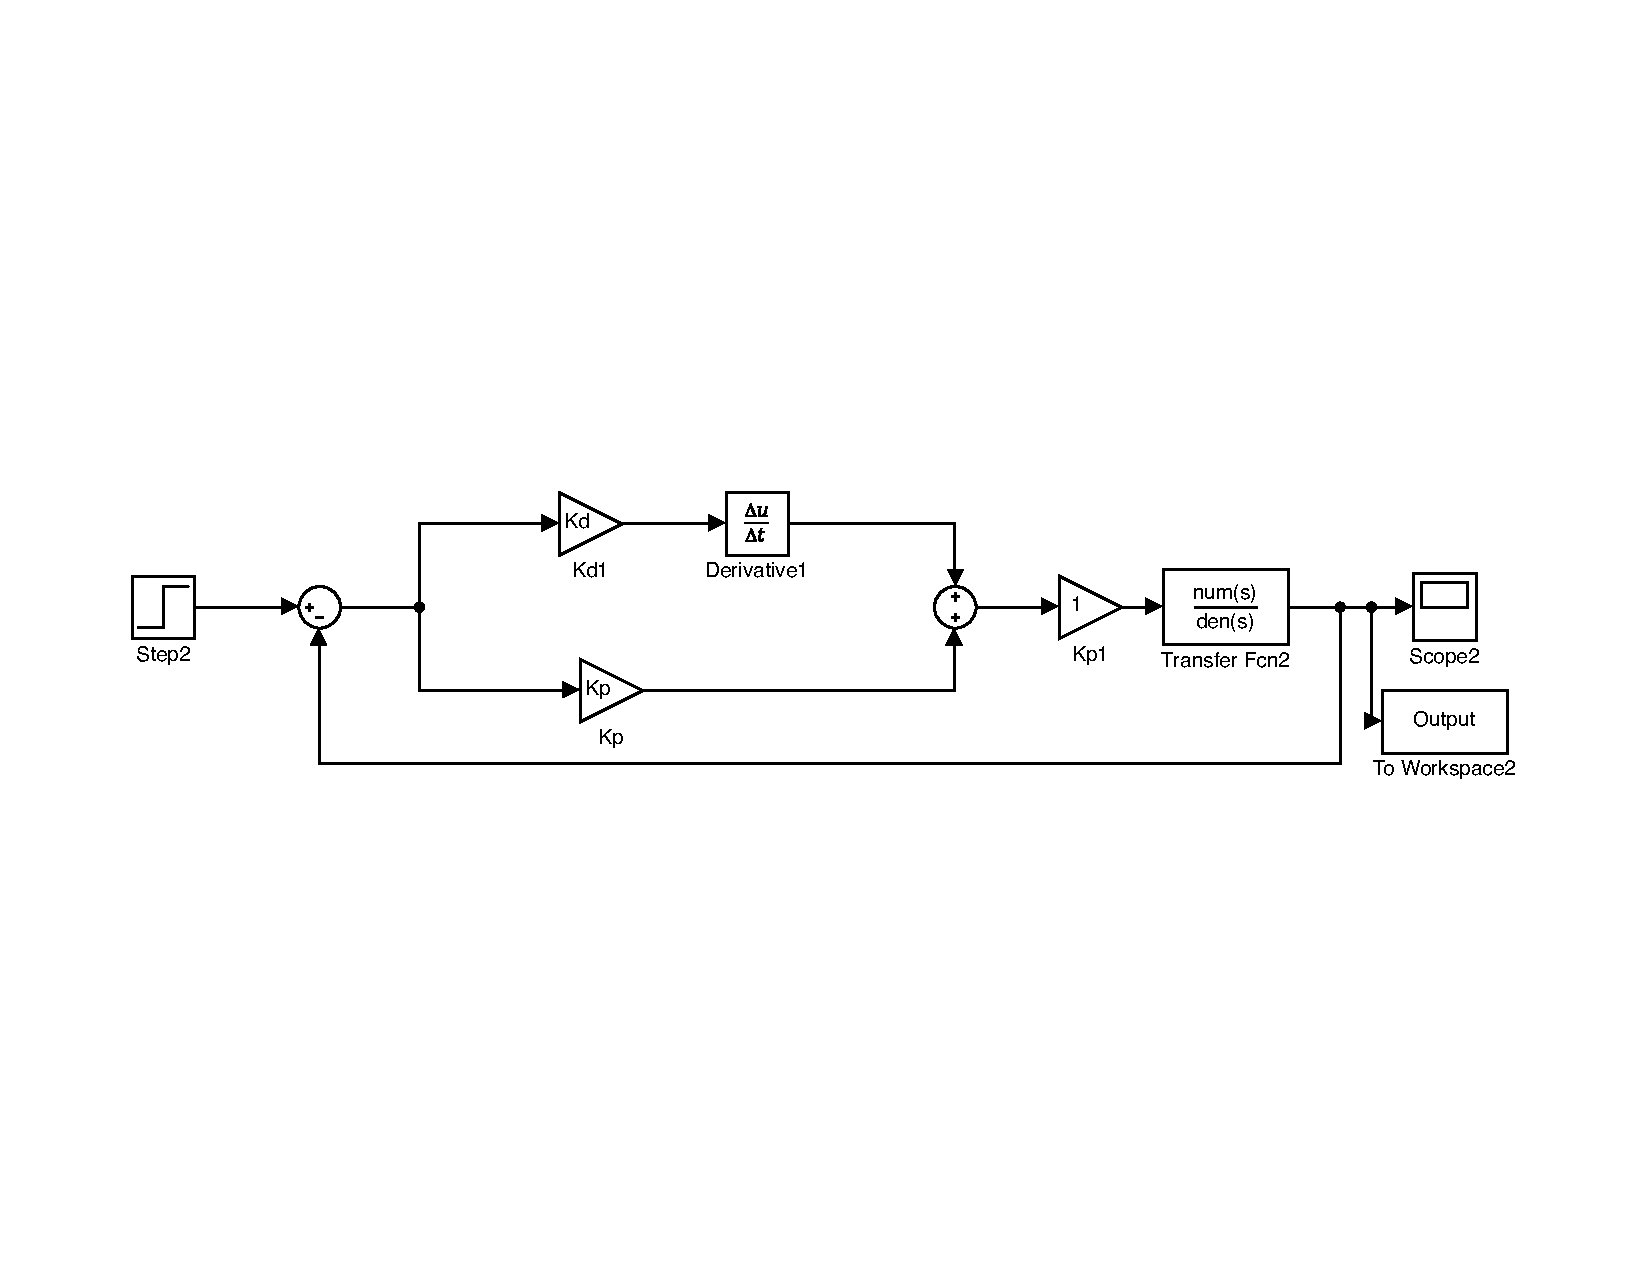
\includegraphics[trim = 0 0 0 0, clip, width=0.59\textwidth]{pd2.pdf}
\vspace{-10pt}
\caption{PD Feedback Controller}
\label{pd2}
\vspace{-20pt}
\end{wrapfigure}

Derivative control utilises the expected \emph{Future} state of the
system to pre-emptively correct the error signal, \(e\). This correction
is proportional to the rate of change of the system state at any one
point in time. The system predict the future plant state based on the
rate of change condition. It then accounts for the effects of this
condition in the error response. For this reason, a large damping effect
is expected for increasing derivative gain (\(K_d\)). The simulation in
Figure \ref{pd2} was implemented to observe the effect of pure variation
of \(K_d\) with constant a \(K_p\). Figure \ref{vkpvkd} shows the effect
of varying both gains by the same magnitude; controlled using an
additional gain block after the controller. Gain values in Figure
\ref{vkpvkd} and Figure \ref{ckpvkd} were incremented from 0 to 1 in
increments of 0.1.

\begin{wrapfigure}{r}{0.45\textwidth}
\centering
\vspace{-15pt} % Space added to the top of the image
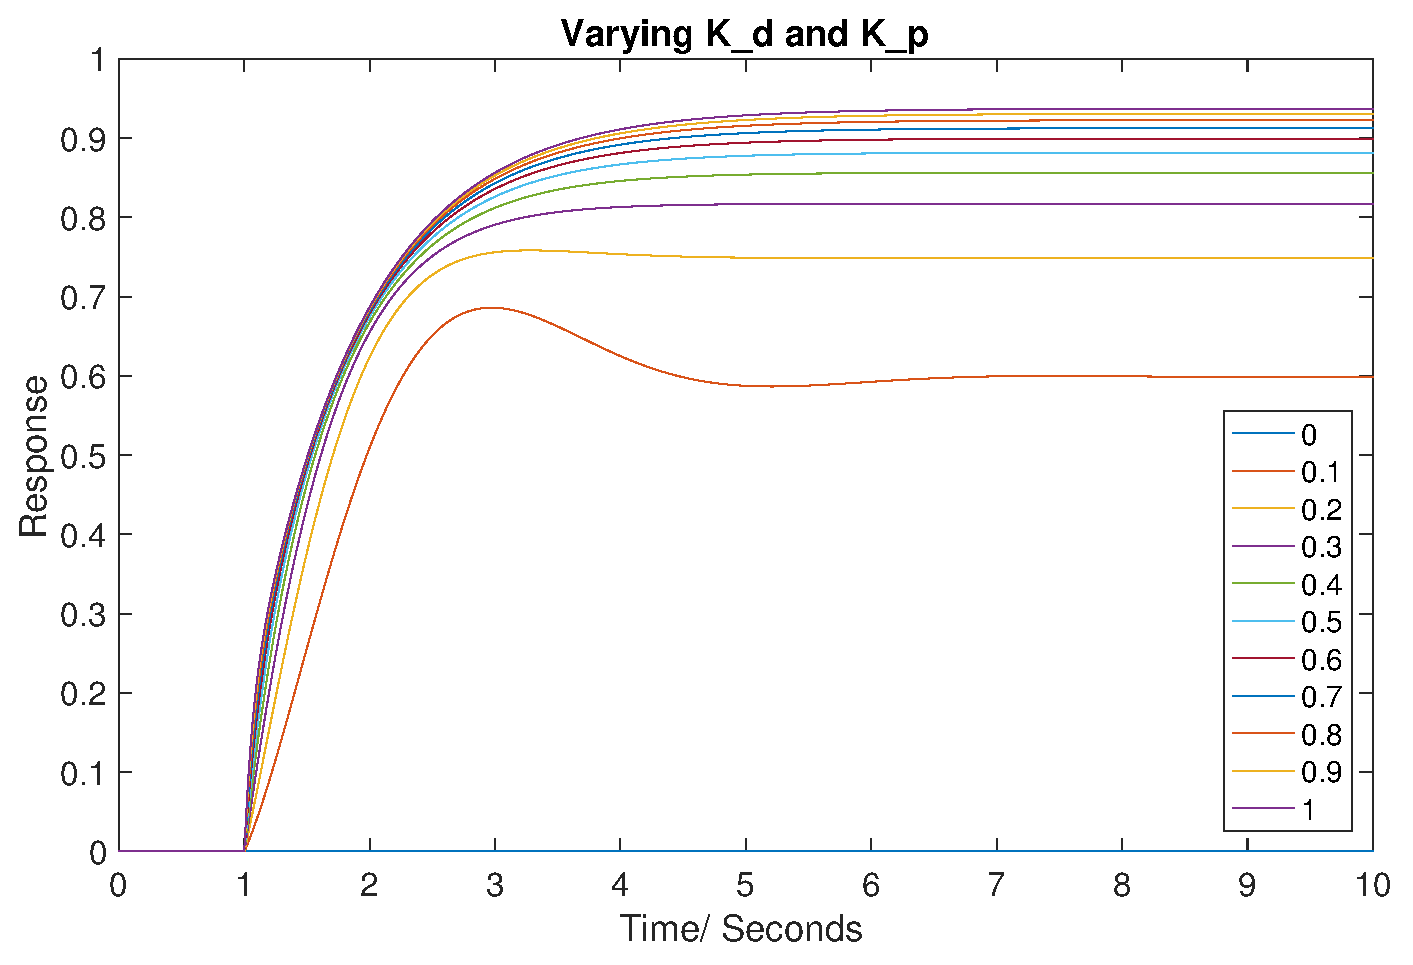
\includegraphics[trim = 0 0 0 0, clip, width=0.45\textwidth]{vkpvkd.eps}
\vspace{-10pt}
\caption{Time-Domain Response For Varying $K_p$ and Varying $K_d$}
\label{vkpvkd}
\vspace{-15pt}
\end{wrapfigure}

Both time domain responses show that increasing \(K_d\) has a greater
damping effect on oscillations, reducing overshoot while increasing rise
time. For a \(K_d = 0\), large oscillations were observed, decreasing
with higher gain values. For gain values of 0.6 and above, both high
damping and quick settling times were observed. Increasing both \(K_d\)
and \(K_p\) by the same amount shows a reduction in rise time, overshoot
and steady-state error. The root locus S-domain metrics in Figure
\ref{pzd} show that as \(K_d\) increases the poles are shifted
negatively in the real axis. The semi-circular shape represents the line
of equal proportional gain, and the points represent varying \(K_d\) at
that \(K_p\) level. As \(K_d\) is increased, the polar angle also
increases. This implies poles closer to the real axis, (higher \(K_d\))
correspond to poles with greater damping; the natural frequency is
therefore reduced, decreasing oscillatory behaviour.

\begin{figure}[H]
\centering
\begin{minipage}{.455\textwidth}
 \centering
 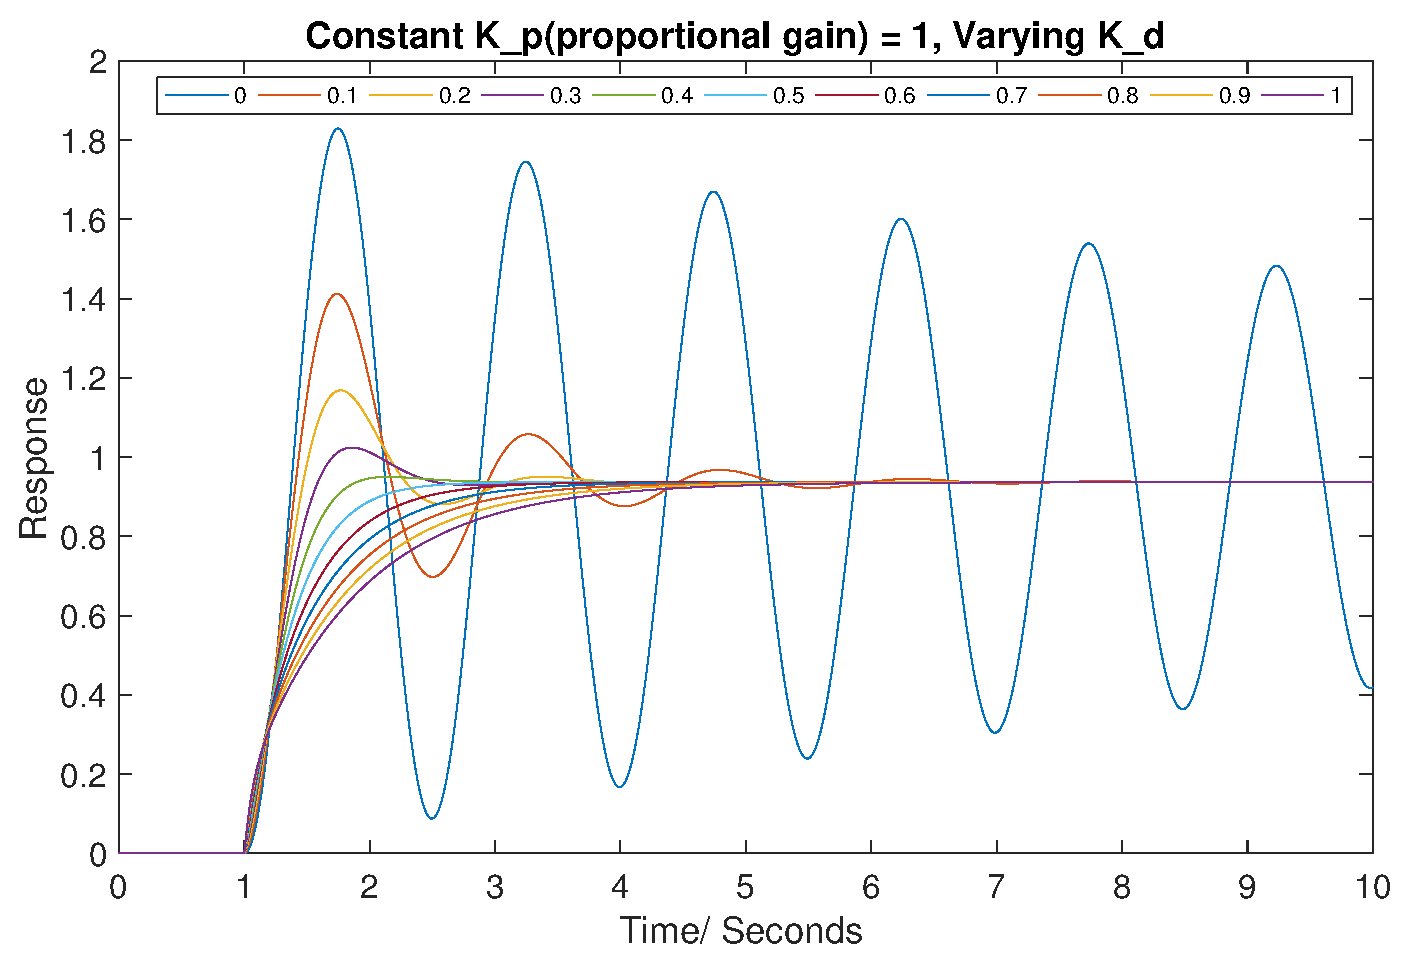
\includegraphics[trim = 0 0 0 0, clip, width=1\textwidth]{ckpvkd.eps}
 \caption{Time-Domain Response For Constant $K_p$ and Varying $K_d$}
 \label{ckpvkd}
\end{minipage}
\hfill
\begin{minipage}{.455\textwidth}
\centering
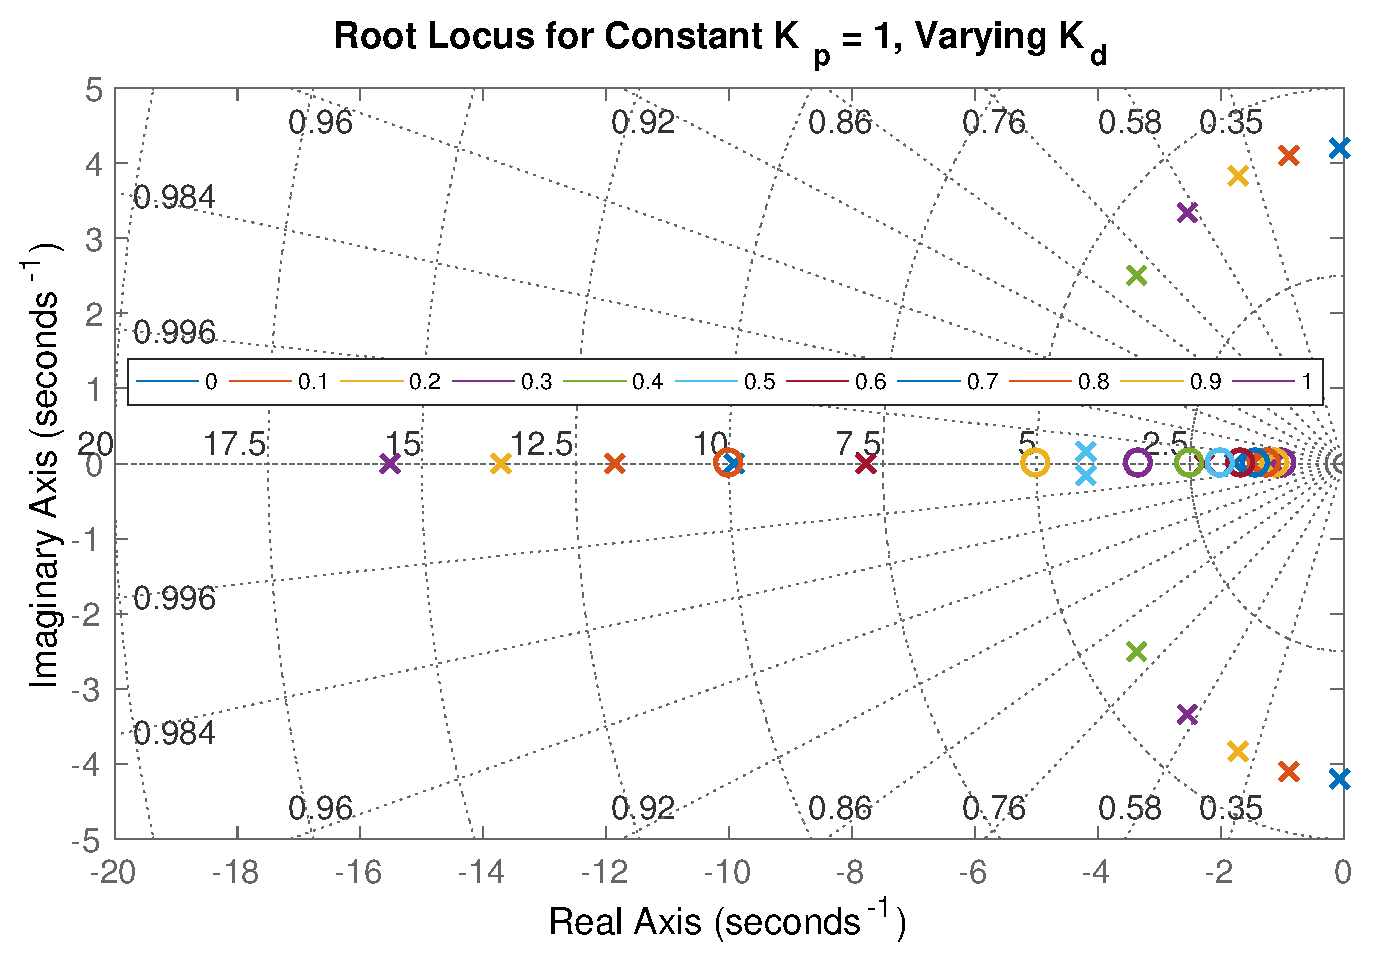
\includegraphics[trim = 0 0 0 0, clip, width=1\textwidth]{pzd.eps}
\caption{Poles of Constant $K_p$ and Varying $K_d$}
\label{pzd}
\end{minipage}
\vspace{-20pt}
\end{figure}

\subsection{Integral Action}\label{integral-action}

\begin{wrapfigure}{r}{0.5\textwidth}
\centering
\vspace{-35pt} % Space added to the top of the image
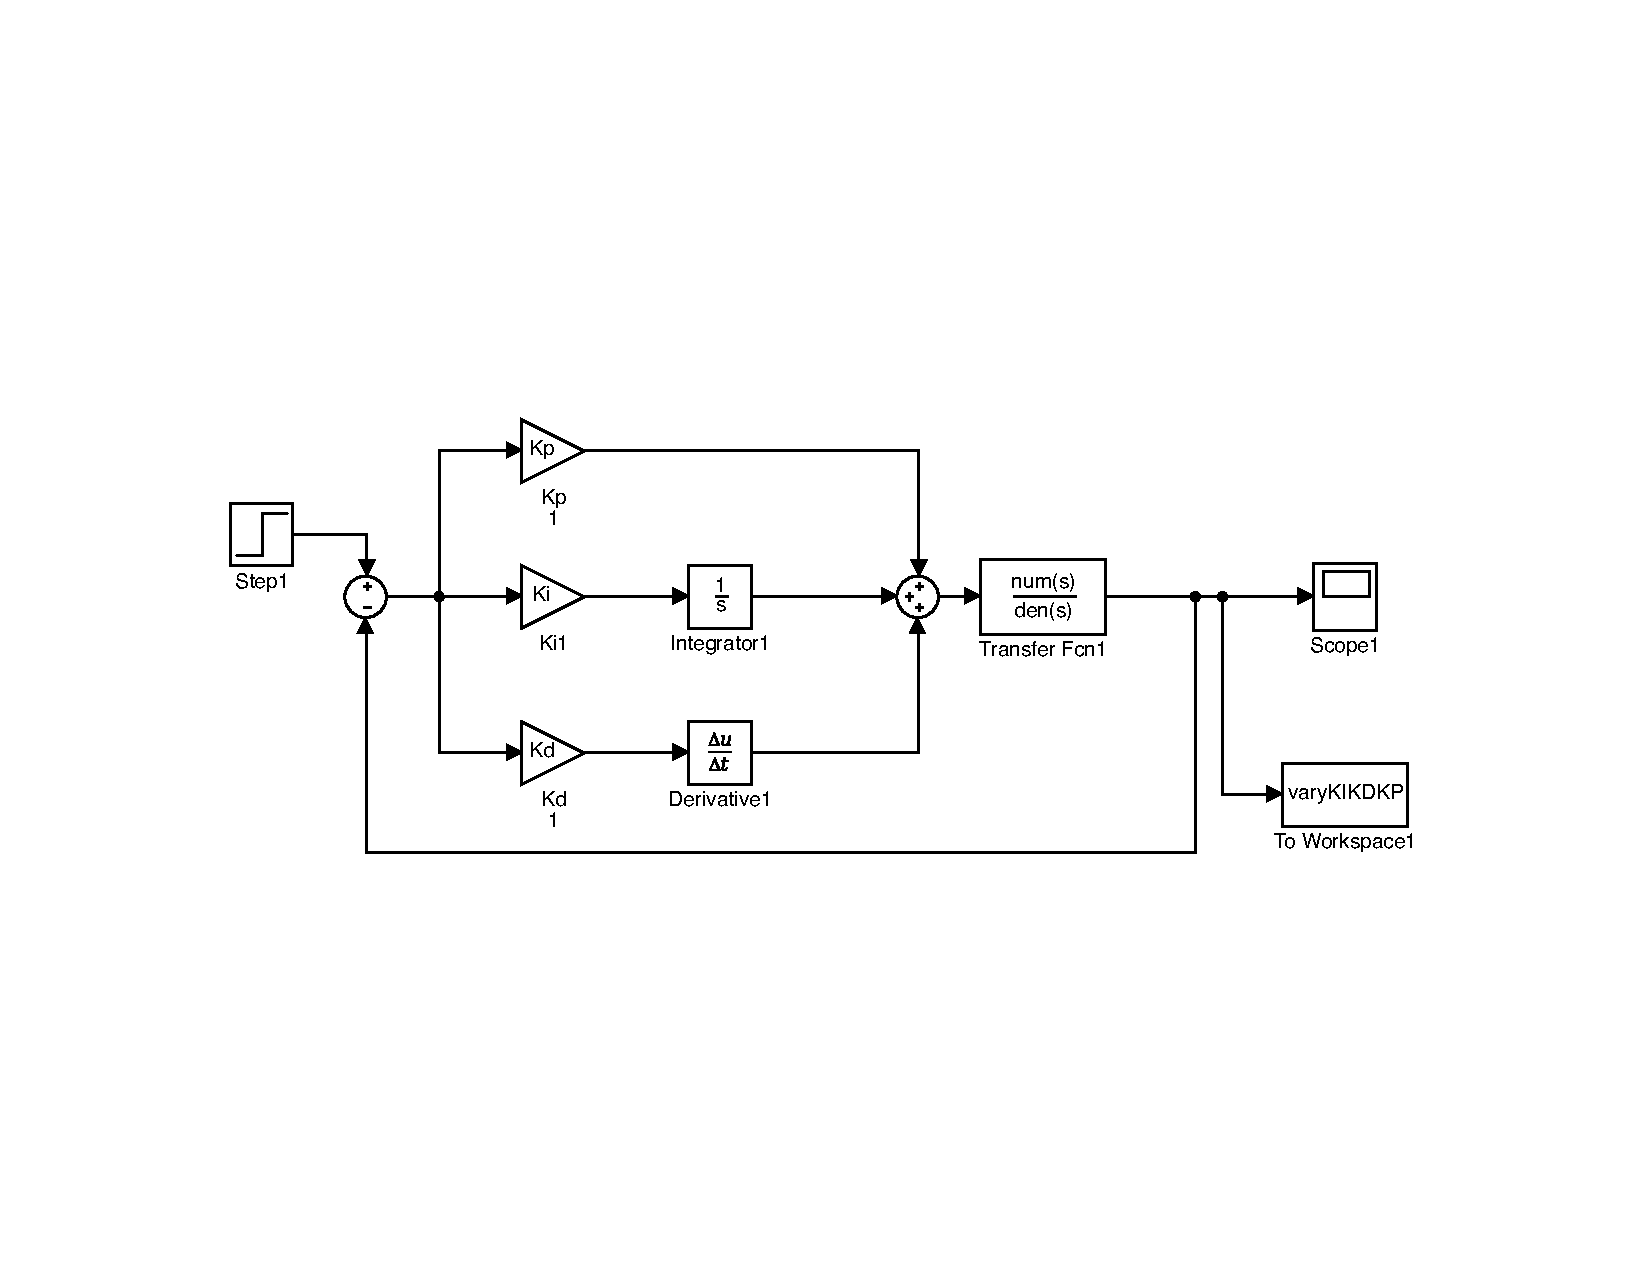
\includegraphics[trim = 0 0 0 0, clip, width=0.5\textwidth]{PIDp2.pdf}
\vspace{-15pt}
\caption{PID Feedback Controller}
\label{PIDp2}
\vspace{-15pt}
\end{wrapfigure}

Integral control utilises the \emph{Past} state of the system to produce
an error-correcting signal. The integral controller sums the historical
tracking errors up to current time state, eliminating offset and leading
to a zero steady-state error. The simulation of a full PID controller is
shown in Figure \ref{PIDp2}. Figure \ref{ckpckdvki} shows the variation
of pure integral gain (\(K_i\)) with constant \(K_p\) and \(K_d\).
Figure \ref{vkpvkdvki} shows the variation of all three gains \(K_d\),
\(K_i\) and \(K_p\) by the same magnitude. This was implemented using a
gain-scaling block placed after the controller. The time domain plots
confirm the zero steady-state error as the oscillations settled at unity
step input.

\begin{figure}[h]
\centering
\begin{minipage}{.465\textwidth}
 \centering
 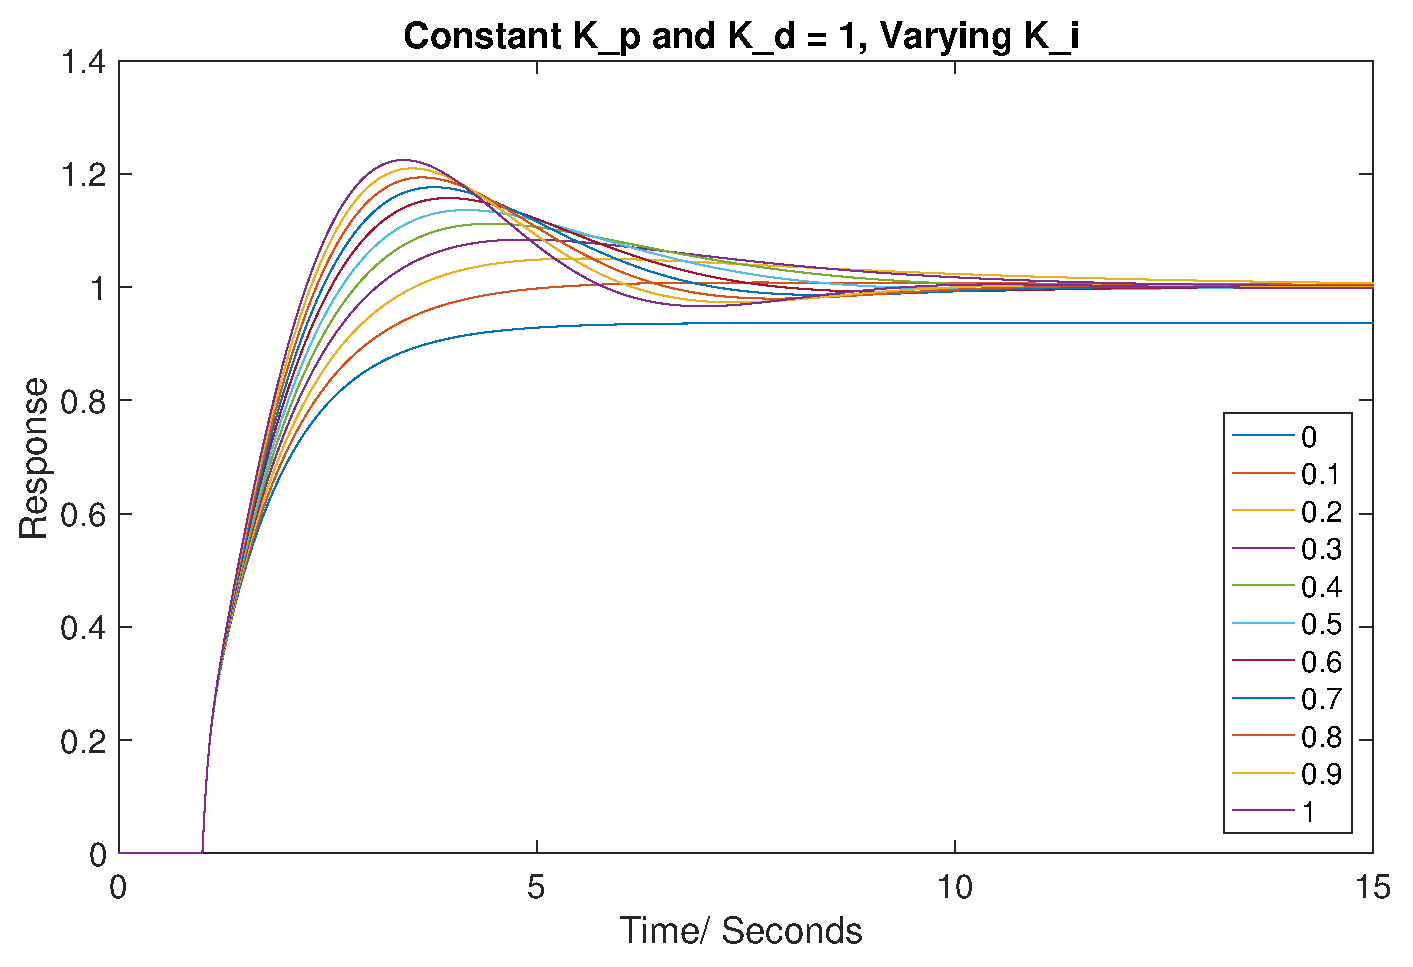
\includegraphics[trim = 0 0 0 0, clip, width=1\textwidth]{ckpckdvki.eps}
 \caption{Time-Domain Response For Constant $K_p$, $K_d$ and Varying $K_i$}
 \label{ckpckdvki}
\end{minipage}
\hfill
\begin{minipage}{.465\textwidth}
\centering
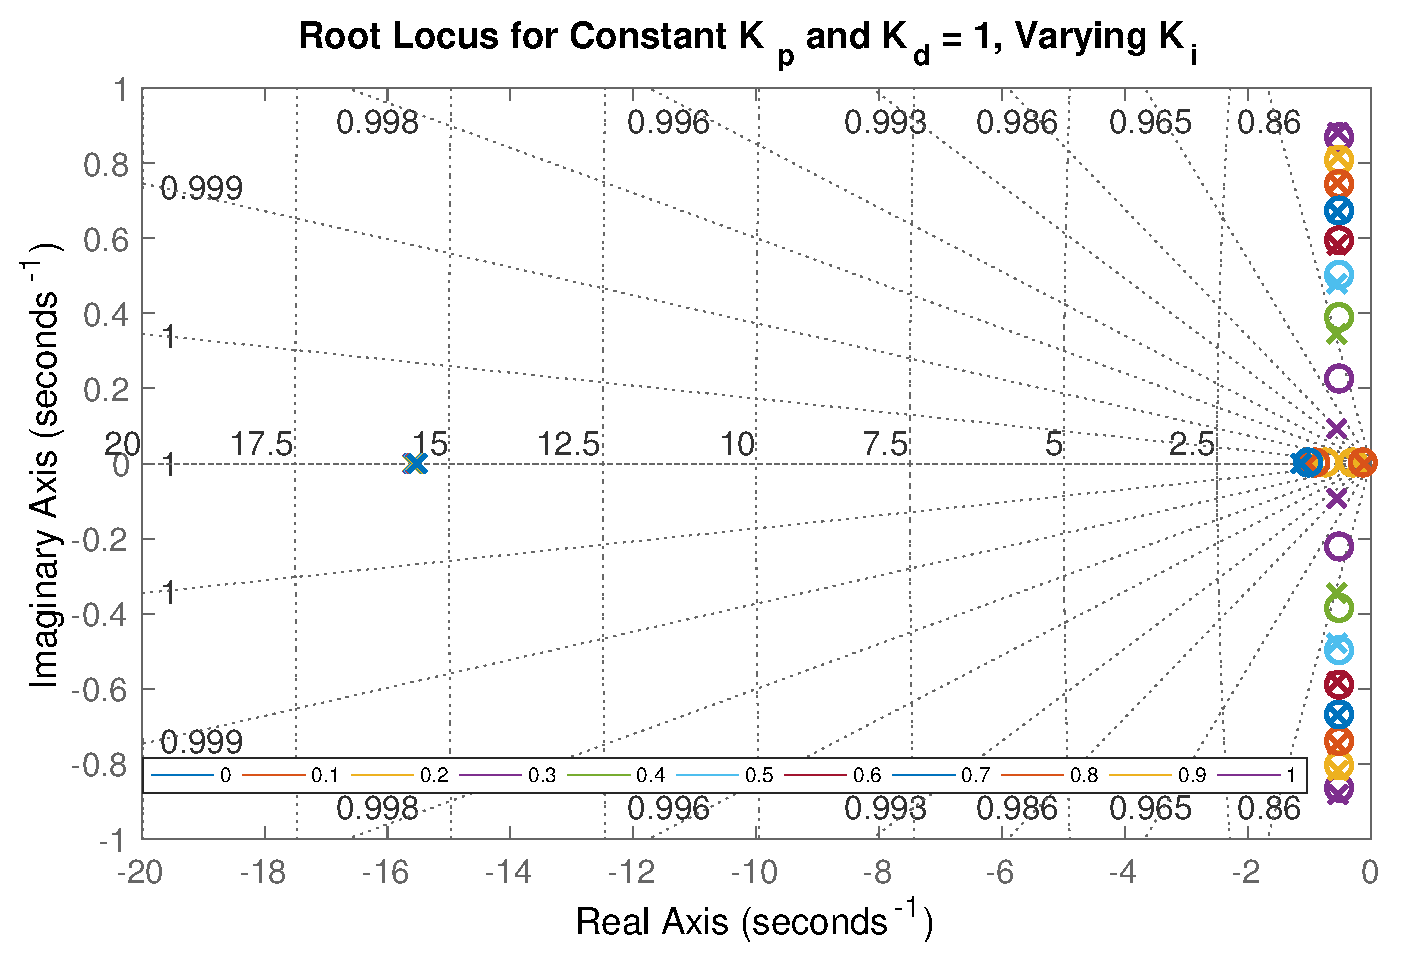
\includegraphics[trim = 0 0 0 0, clip, width=1\textwidth]{pzi.eps}
\caption{Poles of Constant $K_p$, $K_d$ and Varying $K_i$}
\label{pzi}
\end{minipage}
\vspace{-15pt}
\end{figure}

\begin{wrapfigure}{r}{0.5\textwidth}
\centering
\vspace{-5pt} % Space added to the top of the image
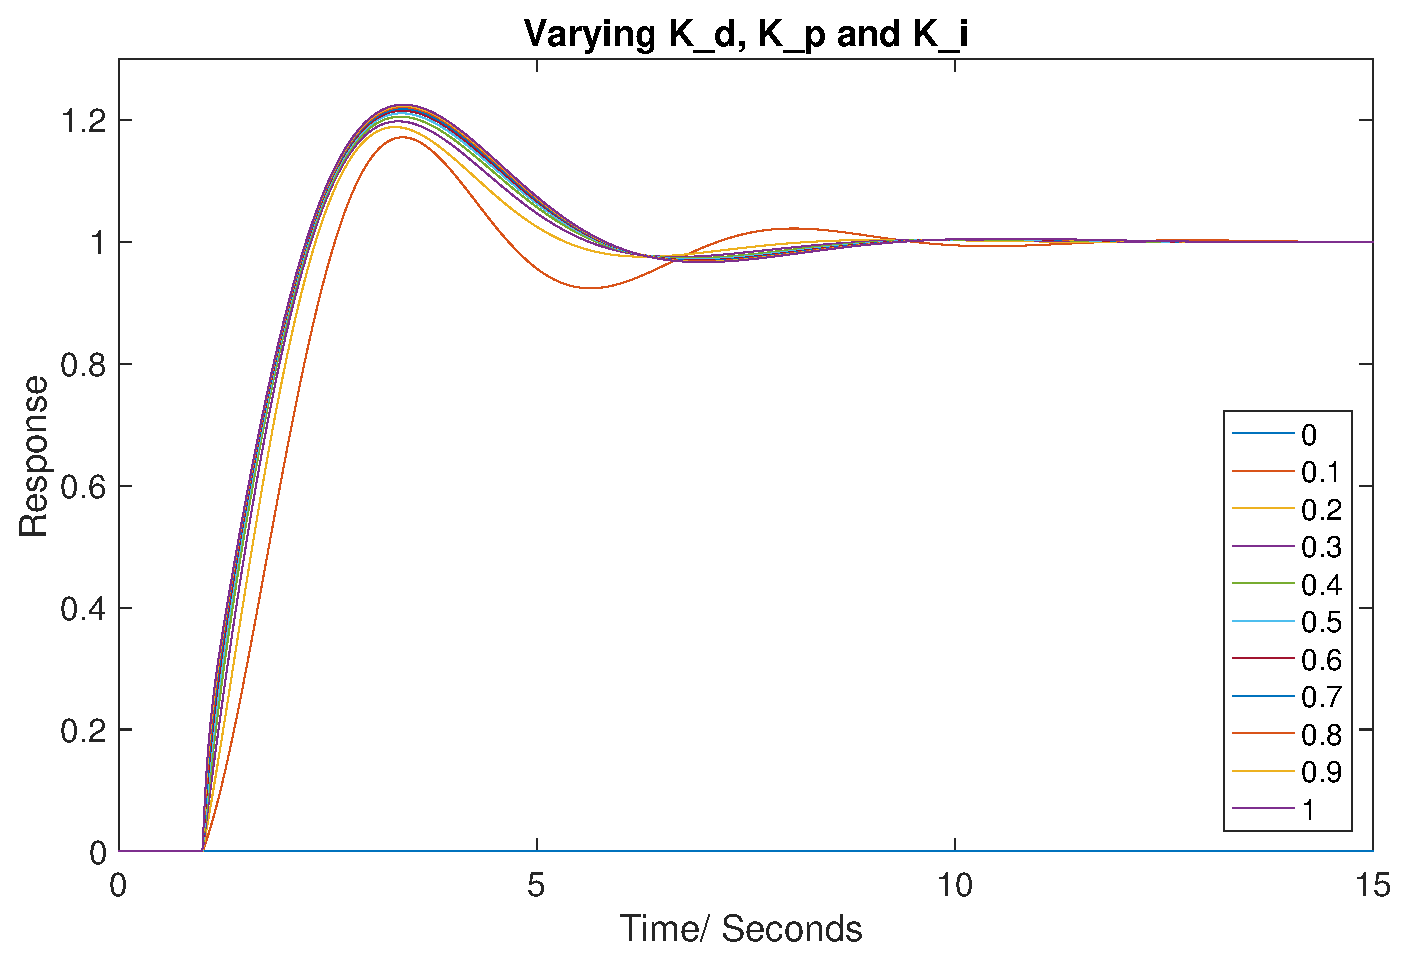
\includegraphics[trim = 0 0 0 0, clip, width=0.5\textwidth]{vkpvkdvki.eps}
\vspace{-10pt}
\caption{Time-Domain Response For Varying $K_p$, $K_d$ and $K_i$}
  \label{vkpvkdvki}
\vspace{-35pt}
\end{wrapfigure}

At \(K_i = 0\) a large steady-state error exists in the system. However
as \(K_i\) increases, the steady state error is reduced until it becomes
negligible. The root locus plot in Figure \ref{pzi}, implies a stable
system for the chosen gain range.

Observing the three controllers, for Quanser elevation, it is important
to have a behaviour with a very low steady-state error and damped
oscillations. This is due to a Quanser pilot requiring precise
elevation, particularly at landing and taking off. Based on these
requirements a PID controller appears to be the most appropriate
feedback method for the Quanser's elevation response transfer function.

\section{PID Design to Achieve Control
Requirements}\label{pid-design-to-achieve-control-requirements}

\begin{wraptable}{r}{0.5\textwidth}
\vspace{-20pt}
\caption{Effect of Increasing PID Gains on Objectives}
\vspace{-5pt}
\centering
 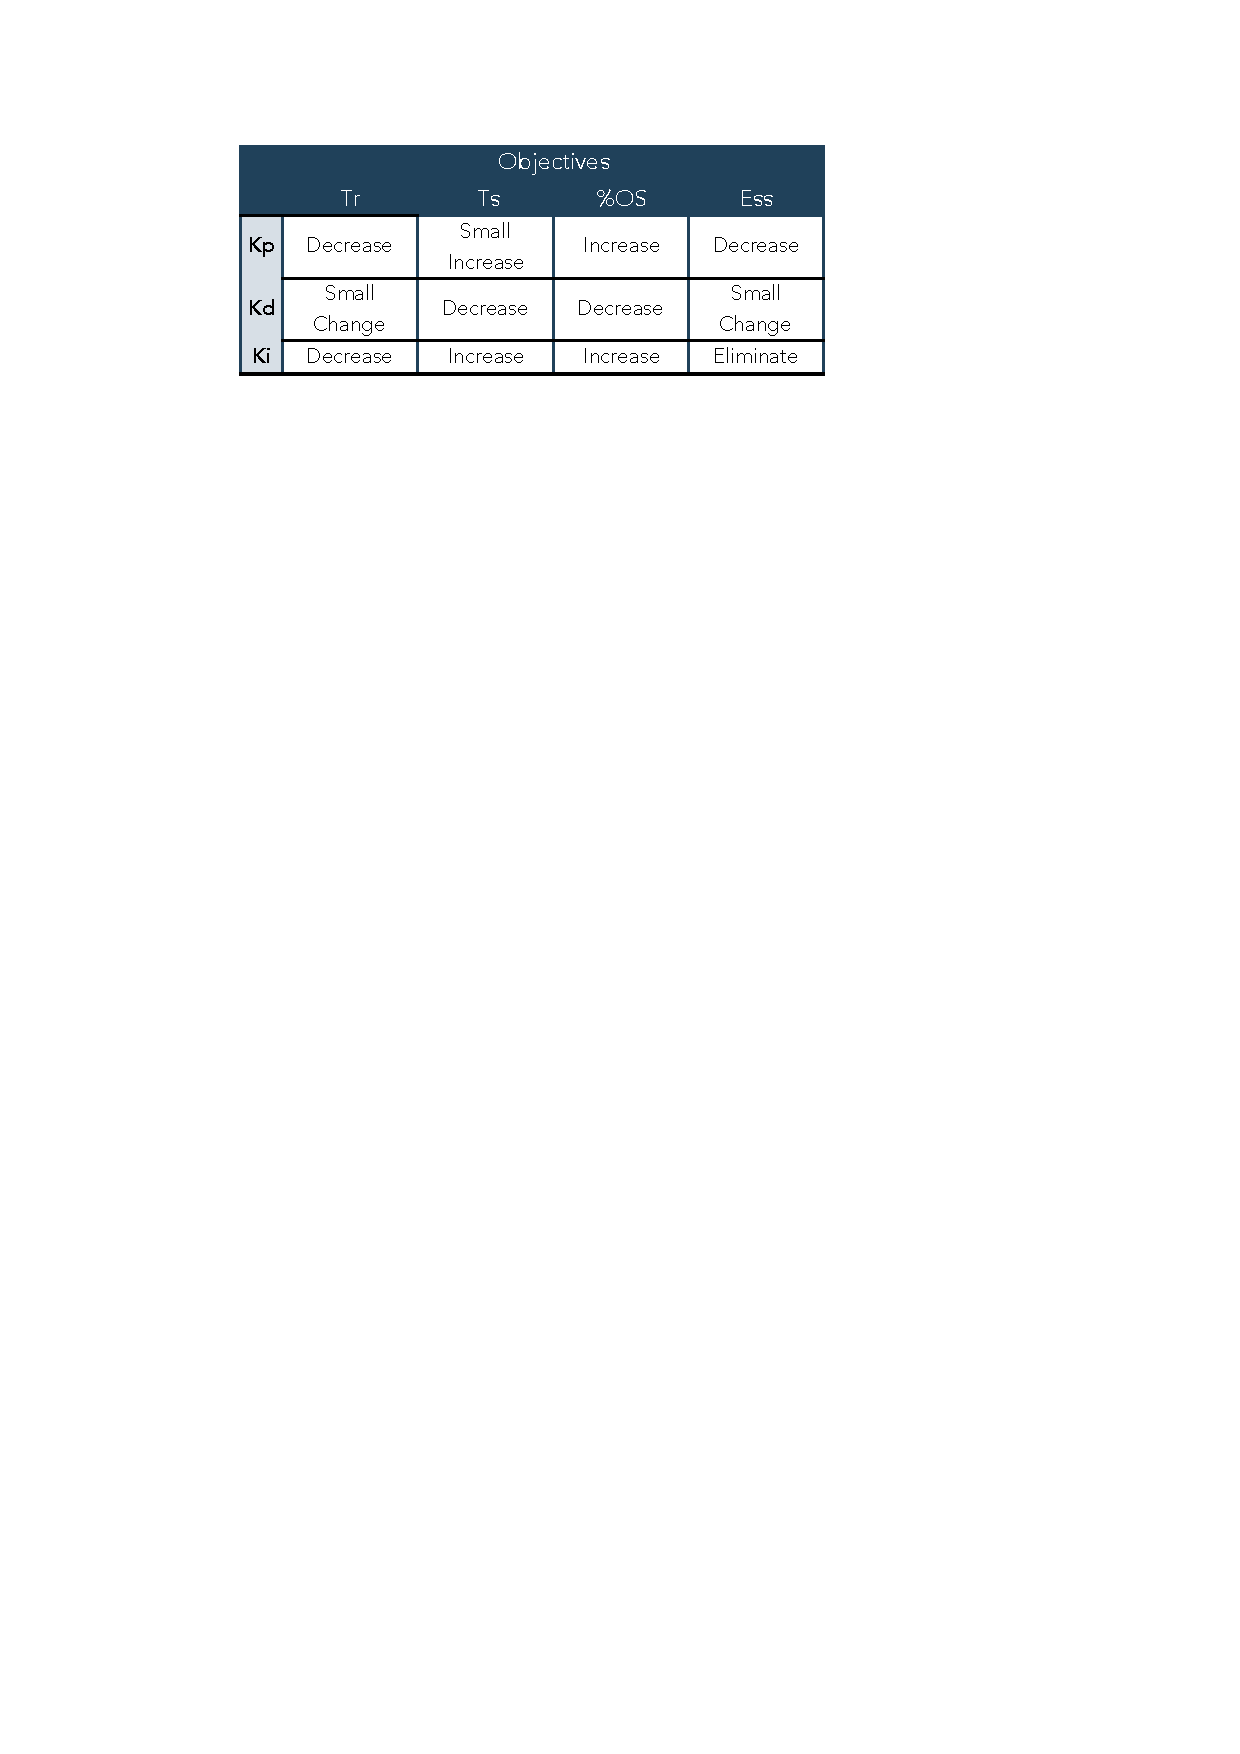
\includegraphics[trim = 0 0 0 0, clip, width=0.49\textwidth]{tableobj.pdf}
 \vspace{-20pt}
 \label{paramtab}
\end{wraptable}

Through implementing the learning gained in part 1, a closed
loop-feedback controller was then developed for the theoretical Quanser
transfer functions (see below)
\footnote{The first order transfer function obtained in Control part 1, was corrected using the $\tau$. $\tau = \zeta \times \omega_n$}.
This controller was tuned, through creating a script which produced the
step response of the controller, displaying results using the
\texttt{stepinfo()} function. Due to the steady state error response
observed through using either a P or PD controller, it was decided to
iterate different gains for using a full PID controller, to obtain the
optimum response. Initially all gains were iterated using the
gain-scaling block (discussed in section \ref{integral-action}). Through
observing the different responses, a rough estimate was found for all
three gains, which could then be individually tweaked based on the
parameters shown in Table 1. Results were also refined using Matlab's
inbuilt PID tuner, helping rise and settling time objectives.

\begin{align*}
&\text{$2^{nd}$ Order: }k \cdot \frac { 1.109\cdot \frac{180} {\pi} }{ s^2 + 0.1313s +1.109 }
&&\text{$1^{st}$ Order: }k \cdot \frac { 1 }{ 15.24s +1 }
\end{align*}

\subsection{PID Controller Tuning}\label{pid-controller-tuning}

As the proportional, integral and derivative gain values were adjusted
to tune the PID, the characteristics for changing each gain were
considered with reference to Table 1. The controller was then tuned as
necessary to best meet the requirements. Analysing the first order
transfer function response, a high rise and settling time were both
observed. As the Quanser behaves as a second order system, it was
decided to neglected the first order transfer function in favour of the
second order transfer function. The tuned response can be seen in Figure
\ref{p2atun}.

\begin{figure}[H]
\centering
\begin{minipage}{.5\textwidth}
 \centering
 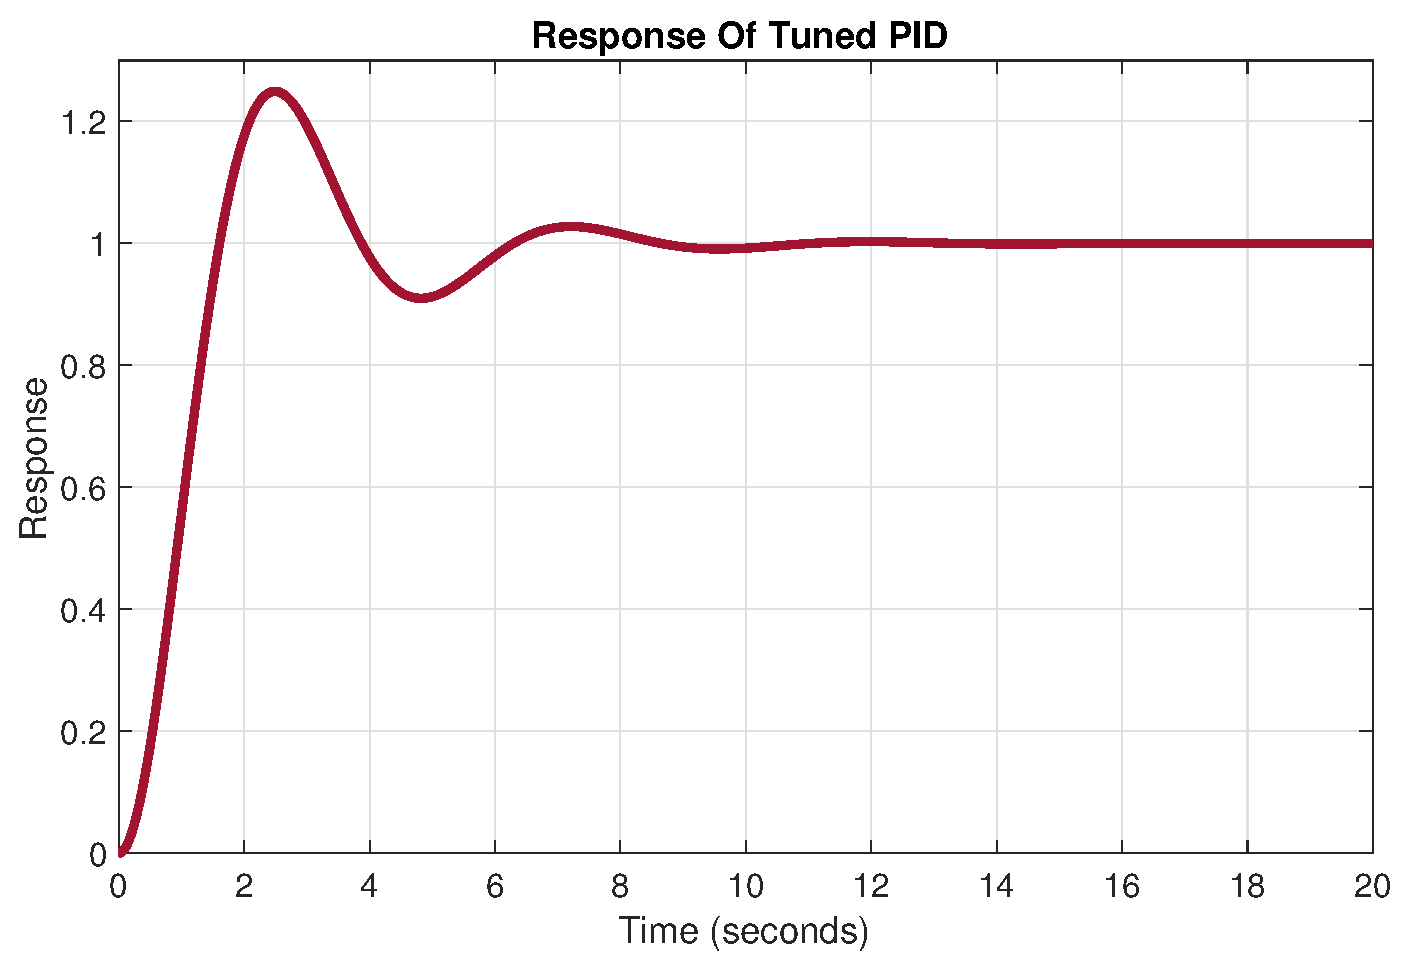
\includegraphics[trim = 0 0 0 0, clip, width=1\textwidth]{p2atun.eps}
 \vspace{-20pt}
 \ \captionof{figure}{Tuned PID Response}
 \label{p2atun}
\end{minipage}
\hfill
\begin{minipage}{.35\textwidth}
\centering
\captionof{table}{Tuned PID Transfer Function Values}
\vspace{-10pt}
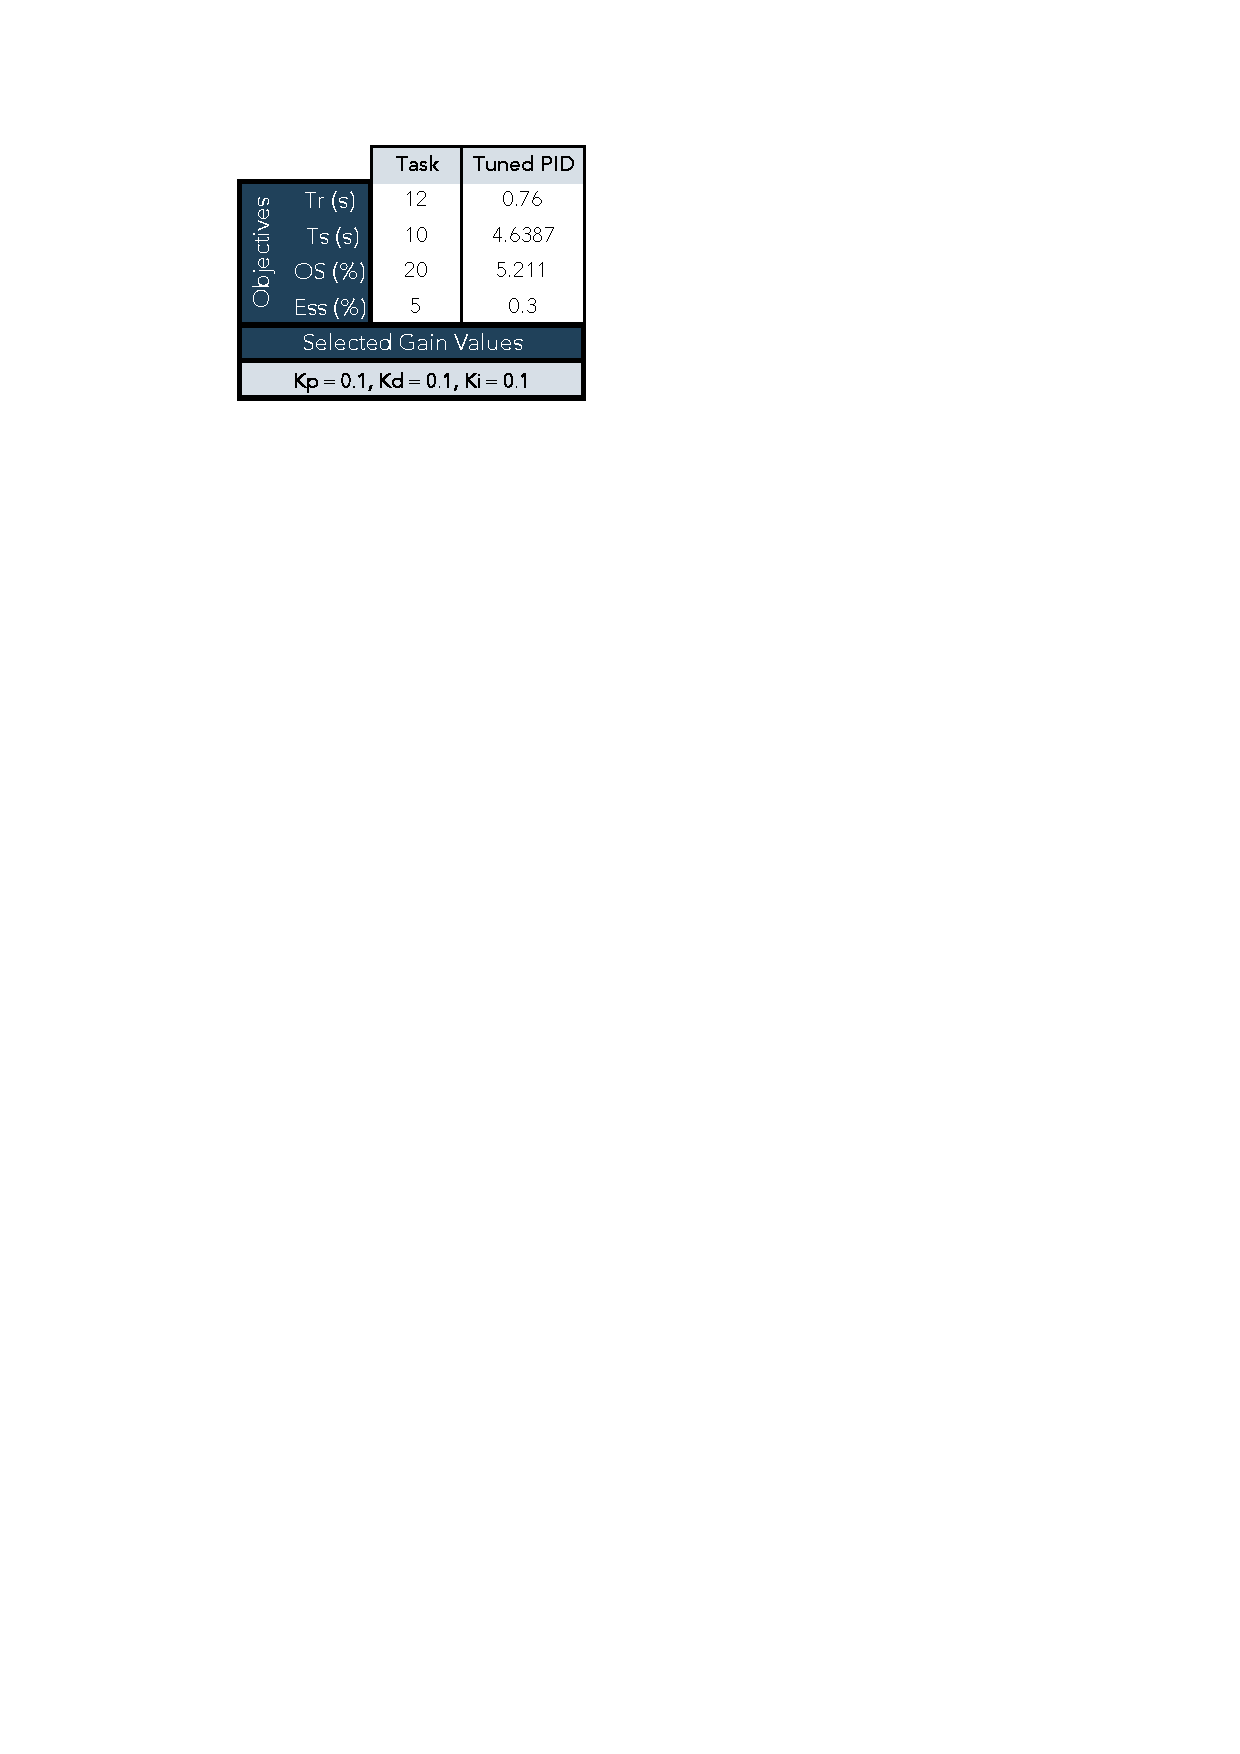
\includegraphics[trim = 0 0 0 0, clip, width=1\textwidth]{paramtuned.pdf}
\label{paramtab}
\end{minipage}
\vspace{-20pt}
\end{figure}

\subsection{Tuned Quanser Controller}\label{tuned-quanser-controller}

A PID controller with the stated \(K_p\), \(K_d\), and \(K_i\) values
was created inside the \texttt{SSC17\_QuanserPart2\_PID}
\texttt{design.slx} controller block. The second order transfer function
was placed into the empty \texttt{PLANT} block. The expected Quanser
response then observed for the chosen PID and plant configurations. In
addition the two other \texttt{EXTREME} plants were tested to ensure the
controller was working effectively. Figure \ref{p2bres} shows the design
configuration response due to step input as well as the extreme plant
response to the designed controller.

\begin{figure}[H]
\centering
\begin{minipage}{.495\textwidth}
 \centering
 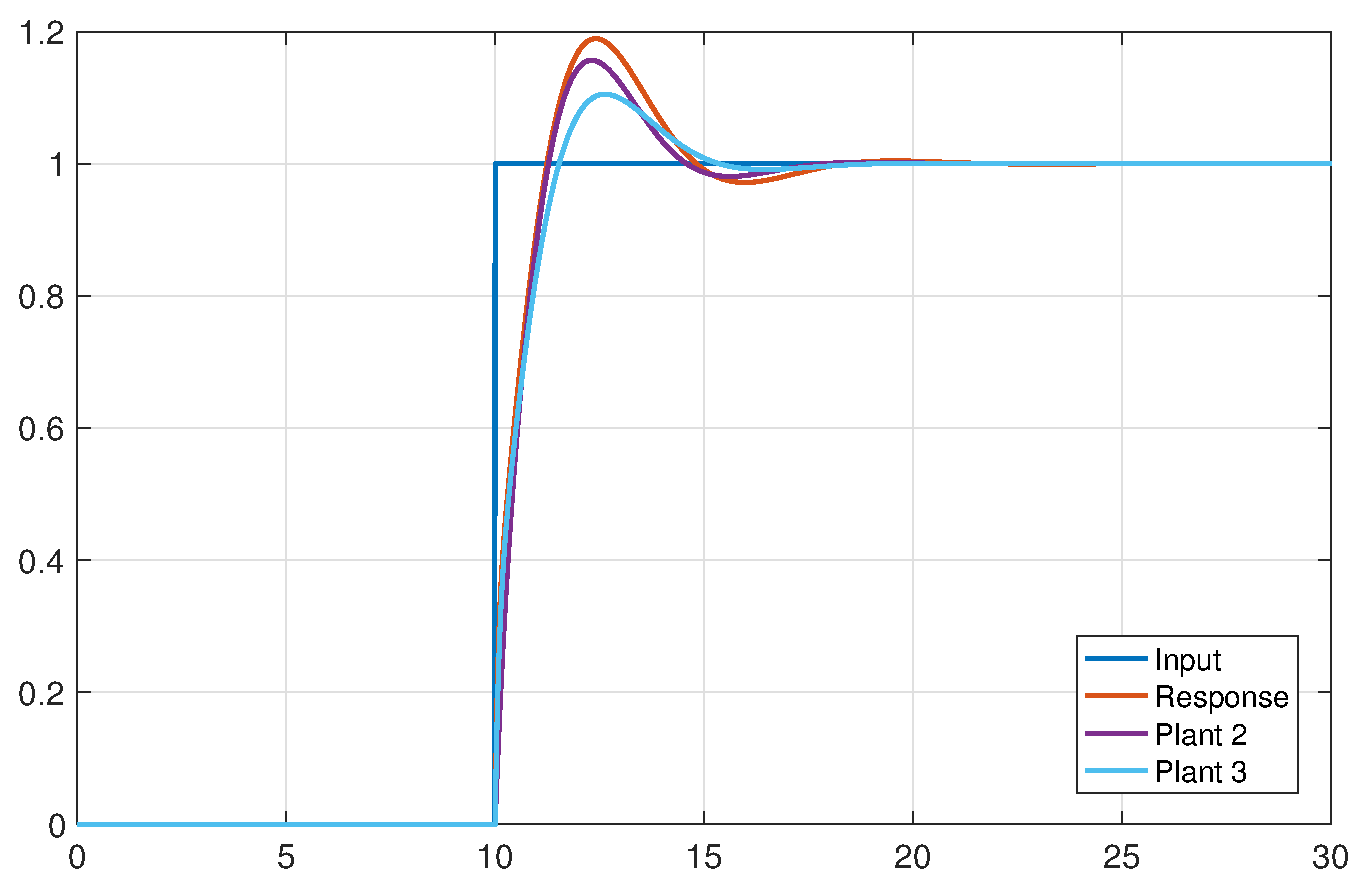
\includegraphics[trim = 0 0 0 0, clip, width=1\textwidth]{p2bres.eps}
 \vspace{-20pt}
 \caption{Expected Quanser Repsonse of PID Controller}
 \label{p2bres}
\end{minipage}
\hfill
\begin{minipage}{.495\textwidth}
\centering
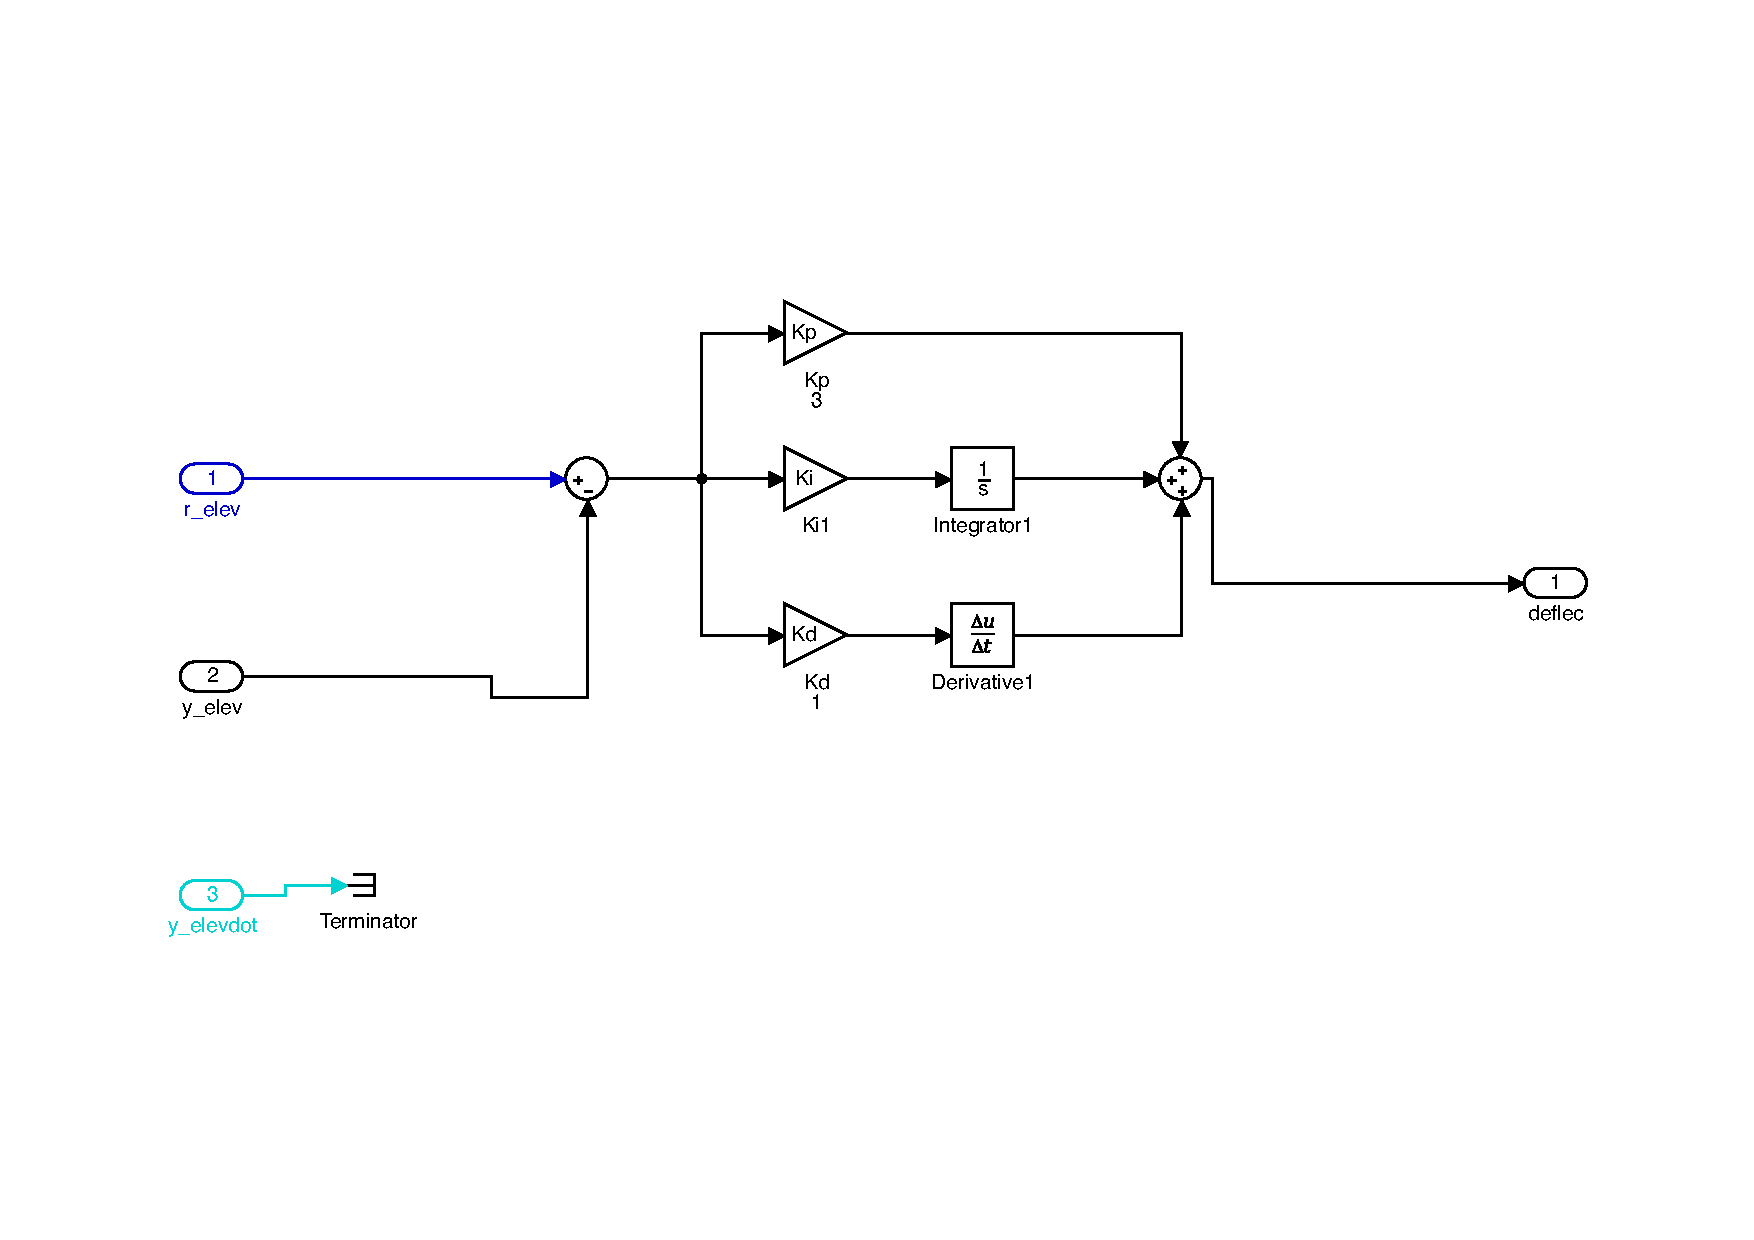
\includegraphics[trim = 0 0 0 0, clip, width=1\textwidth]{theorycontr.pdf}
\vspace{-10pt}
\caption{Simulation Used for Theory Controller}
\label{paramtab}
\end{minipage}
\vspace{-20pt}
\end{figure}
% -----------------------------------------------------------------------------------
%                                  APENDIX
% -----------------------------------------------------------------------------------

\end{counted} %<<<<<<<<<<<<<<ENDS WORD COUNTER

% \newpage
% % \section{Appendices}
% Above were \thewords\ words. %<<<<<<<<<<<<<<DISPLAYS WORD COUNTER
% -----------------------------------------------------------------------------------
%                               BIBLIOGRAPHY - Insert Name of BIB File Here
% -----------------------------------------------------------------------------------
% \newpage

% ---------------BIBTEX OLD-----------------------------------------------------
% \bibliographystyle{unsrt} %%%% Plain or alpha can change orders here
% \bibliography{BibFile}
% \nocite{*} %%%if you want to see all references even those note cited in the text
% -----------------------------------------------------------------------------------

\printbibliography

\end{document}
